\chapter{State of the art system identification analysis}
\label{identification_methods}

\emph{In this chapter, first an overview is given about the different steps that one has to consider in non-linear system identification. Secondly, different approaches are explained and compared. As a conclusion of the comparison, the selected approach is further discussed which leads to the introduction of Artificial Neural Networks(ANNs). Afterwards, the system identification and validation is carried out using the available data from the EPANET framework.}

\section{Tasks in non-linear system identification}
\label{tasks_nonlinear_sys_identification}

Modelling and identification of non-linear systems is a challenging task because non-linear processes do not share properties such as the superposition in linear systems. In this sense, non-linear systems are unique and the methods for describing structurally different systems are complex. However, as for any identification method, the goal is to find a model which is capable to represent the behaviour of a process as closely as possible. The quality of the model is typically measured in terms of the error between the output of the process and the model. In \figref{fig:nonlin_block} an illustration is shown for a system identification arrangement 
\vspace{-3mm}
 %Non-lin system identification 
\begin{figure}[H]
\centering
%
\includegraphics[width=0.35\textwidth]{report/pictures/missingfigure}
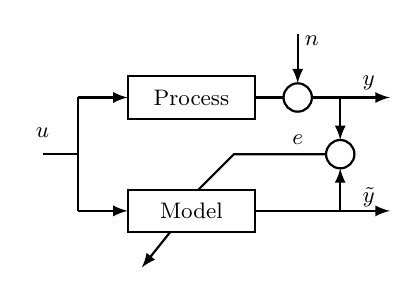
\begin{tikzpicture}[scale=0.9,transform shape]

\draw [thick] (-3,3) rectangle (-1.2,2.4);
\node at (-2.1,2.7) {\small Process};
\node at (-2.1,1.1) {\small Model};
\node at (-4.2,2.2) {\small $u$};
\node at (-0.4,3.5) {\small $n$};
\node at (-0.6,2.1) {\small $e$};
\node at (0.4,1.3) {\small $\tilde{y}$};
\node at (0.4,2.9) {\small $y$};


\draw [thick] (-3,1.4) rectangle (-1.2,0.8);
\draw [thick] (-0.6,2.7) ellipse (0.2 and 0.2);
\draw [thick] (0,1.9) ellipse (0.2 and 0.2);
\draw [thick][-latex](-0.4,2.7) -- (0.7,2.7);
\draw [thick][-latex](0,2.7) -- (0,2.1);
\draw [thick][-latex](-1.2,1.1) -- (0,1.1) -- (0,1.7);
\draw [thick](-0.2,1.9) -- (-1.5,1.9) -- (-2,1.4);
\draw [thick](-1.2,2.7) -- (-0.8,2.7);
\draw  [thick][-latex](-2.4,0.8) -- (-2.8,0.3);
\draw  [thick][-latex](0.0,1.1) -- (0.7,1.1);
\draw [thick][-latex](-3.7,2.7) -- (-3,2.7);
\draw [thick][-latex](-3.7,1.1) -- (-3,1.1);
\draw [thick](-3.7,2.7) -- (-3.7,1.1);
\draw [thick](-4.2,1.9) -- (-3.7,1.9);
\draw  [thick][-latex](-0.6,3.6) -- (-0.6,2.9);
\end{tikzpicture} 
\vspace{-3mm}
\caption{Block diagram of system identification.}
\label{fig:nonlin_block}
\end{figure}

\vspace{-4mm}

The process and model are fed with the same input signals, and their outputs are compared. This comparison gives an error signal $e$, which can be utilized for adapting the model. It should be noted, that in most cases the measurements on the output are disturbed by noise $n$. In order to carry out a succesful system identification, some major steps need to be performed, either by user interaction or using algorithms which can automatize these steps. \figref{fig:identification_loop} shows the system identification loop with the major steps

 %system identification algorithm 
\begin{figure}[H]
\centering
%
\includegraphics[width=0.35\textwidth]{report/pictures/missingfigure}
\usetikzlibrary{arrows}
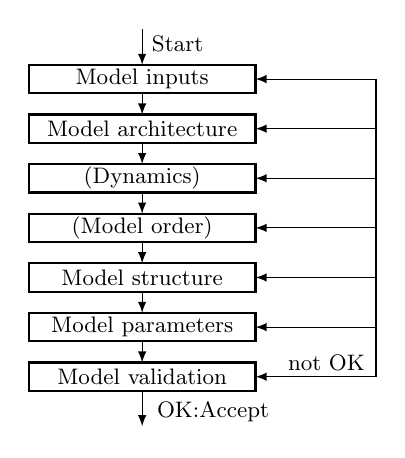
\begin{tikzpicture}[scale=0.9,transform shape]

\draw [thick] (-9.7,6.2) rectangle (-6.5,5.8);
\draw [thick] (-9.7,5.5) rectangle (-6.5,5.1);
\node at (-8.1,6) {\small Model inputs};

\node at (-8.1,5.3) {\small Model architecture};
\node at (-8.1,4.6) {\small (Dynamics)};
\node at (-8.1,3.9) {\small (Model order)};
\node at (-8.1,3.2) {\small Model structure};
\node at (-8.1,2.5) {\small Model parameters};
\node at (-8.1,1.8) {\small Model validation};
\node at (-7.6,6.5) {\small Start};
\node at (-7.1,1.3) {\small OK:Accept};
\node at (-5.5,2) {\small not OK};

\draw [thick][-latex] (-9.7,4.1) rectangle (-6.5,3.7);
\draw [thick][-latex] (-9.7,4.4) rectangle (-6.5,4.8);
\draw [thick][-latex] (-9.7,3.4) rectangle (-6.5,3);
\draw [thick][-latex] (-9.7,2.7) rectangle (-6.5,2.3);
\draw [thick][-latex] (-9.7,2) rectangle (-6.5,1.6);
\draw [-latex](-8.1,5.8) -- (-8.1,5.5);
\draw [-latex](-8.1,5.1) -- (-8.1,4.8);
\draw [-latex](-8.1,4.4) -- (-8.1,4.1);
\draw [-latex](-8.1,3.7) -- (-8.1,3.4);
\draw [-latex](-8.1,3) -- (-8.1,2.7);
\draw [-latex](-8.1,2.3) -- (-8.1,2);
\draw [-latex](-8.1,1.6) -- (-8.1,1.1);
\draw [-latex](-8.1,6.7) -- (-8.1,6.2);
\draw [thick](-4.8,6) -- (-4.8,1.8);
\draw [-latex](-4.8,6) -- (-6.5,6);
\draw [-latex](-4.8,5.3) -- (-6.5,5.3);
\draw [-latex](-4.8,4.6) -- (-6.5,4.6);
\draw [-latex](-4.8,3.9) -- (-6.5,3.9);
\draw [-latex](-4.8,3.2) -- (-6.5,3.2);
\draw [-latex](-4.8,2.5) -- (-6.5,2.5);
\draw [-latex](-4.8,1.8) -- (-6.5,1.8);
\end{tikzpicture} 
\caption{System identification loop \cite{nelles2013nonlinear}.}
\label{fig:identification_loop}
\end{figure}

\vspace{-3mm}

Some of these steps in \figref{fig:identification_loop} are discussed in the further sections. Furthermore, in the following, the term Training Set(TS) is used to characterize the measurement data that is utilized to carry out the presented identification steps. A TS consists of $N$ input-output pairs such that

\begin{equation}
  \label{training set}
  \mathcal{D} = \{u_i , y_i\}_{i = 1,2, ..., N}.
\end{equation}

\subsection{Choice of the model inputs}
\label{choice_of_the_model_inputs}

The first step in the identification is typically realized by a trial-and-error approach with the help of prior knowledge. In physical systems such as a WSS, the influence of the different variables is quite clear and the inputs can be chosen by the model equations which were presented in \secref{multi_inlet_multi_WT_model}. It should be noted that in more complex systems, where the number of inputs are high and their influence is not so well defined, some data-driven input selection might be very helpful. In this case, using all inputs can lead to extremely high-dimensional approximation problems, which implies the need for a huge number of parameters and increases the training time. Techniques for input data selection such as Principal Component Analysis(PCA) can be utilized in order to decide the relevance of certain inputs on the system. The main drawback of such techniques is that the relevance of an input is dependant only on the input data distribution, therefore sometimes highly relevant inputs are removed \cite{nelles2013nonlinear}.  Other techniques, such as correlation analysis for linear systems or genetic algorithms for non-linear systems can be also utilized, however it is not discussed further in the report, as in our case all inputs are relevant. 

Furthermore, the choice of the input signal requires some prior knowledge about the operation of the system and the purpose of the model. For black box modelling, the measurement data is the most important source of information. The behaviour of the real world system that is not represented in the TS, cannot be described in the model, unless prior knowledge is explicitly incorporated. Therefore, the TS needs to be as representative as possible in order to incorporate the desired operation of the real world system. 
\vspace{-3mm}
\subsection{Choice of the model structure}
\label{choice_of_the_model_architecture}

The choice of the model architecture among many factors, depends on the type of the problem, the intended use, the insight into the real system behaviour, the complexity and the available data. The type of the problem can be for instance the approximation of a static system, or identification of the dynamics. In our case, both of them are considered. The intended use for the model architecture can differ whether the model is to be used for simulation, control, fault detection, etc. Considering the insight, the complexity and the available data, three different modelling approaches can be distinguished\cite{nelles2013nonlinear}. These approaches are compared in \tabref{comparisontable_sysid}. 

\vspace{-3mm}

\begin{center}
    \begin{tabular}{ | >{\centering\arraybackslash}m{1.8cm} | >{\centering\arraybackslash}m{3.6cm} | >{\centering\arraybackslash}m{3.6cm} | >{\centering\arraybackslash}m{3.6cm} |}
    \hline
    \multirow{1}{*}
     & \textbf{White box} & \textbf{Gray box} & \textbf{Black box} \\ 
     \hline
     \multirow{1}{*}
    \textbf{Information sources} & First principles and insights. &  Some insights and some data. & Data and experiments.\\ 
    \hline
      \multirow{1}{*}
    \textbf{Features} & Good understanding, high reliability and scalability. & $\longleftrightarrow$  & Short development time and insight is not required.\\ 
    \hline
      \multirow{1}{*}
    \textbf{Drawbacks} & Well described process is required. & $\longleftrightarrow$ & Not scalable and the accuracy is restricted by the available data.\\ 
    \hline
          \multirow{1}{*}
    \textbf{Application} & Planning, simulation and design for simple processes. & $\longleftrightarrow$ & Only for existing, rather complex processes.\\ 
    \hline
    \end{tabular}
    \captionof{table}{Comparison of system identification modelling approaches\cite{nelles2013nonlinear}.}
    \label{comparisontable_sysid}
\end{center}

As shown in \tabref{comparisontable_sysid}, White box models are completely derived by first principles, i.e., by physical laws. The parameters and equations, describing the whole network can be determined by theoretical modelling, as it was done for our system in \chapref{system_modelling}. Black box models however, are based on measurement data, which means that the model describing the system is developed by the characteristics of the data. In order to carry out a successful Black box modelling, very little insight or prior knowledge is required, however it is important to have a well-describing TS. The combination or compromise between Black and White box models is called Gray box modelling. In this case, the knowledge from first principles and the information contained in the measurement data are both utilized. The blank fields in \tabref{comparisontable_sysid} for Grey box models are left blank because the properties of such models lie between White and Black box modelling. Typically, when Grey box modelling is considered, the main goal is to overcome some of the most restrictive factors of the White and Black box approaches for the specific application. For example, some prior knowledge might be incorporated into a Black box model in order to ensure reasonable behaviour\cite{nelles2013nonlinear}. 

Often the structure may be determined by first principles but the model parameters may be estimated from data. It is important to note, that the WSS model presented in \chapref{system_modelling} has been derived by first principles, however due to complexity of the system and the available data, the identification will be carried out by Black box identification and approximation methods. 

\subsection{Model validation}
\label{model_validation}

The easiest type of validation is to check the quality of the model on the TS. If this does not give satisfactory results, the model is not accepted. In this case, it can be either concluded that information is missing from the input or the model is not flexible enough to describe the corresponding input-output relations. In case if the performance achieved on the TS is acceptable, it is desirable to test the model on a new data set, especially if noise is present in the system. It should be noted however, that this new testing data should excite the system in the same operating regions, as the model was trained on. Otherwise, the model fails the validation. 

\newpage

\section{Model structure of the Multi-inlet, Multi-WT system}
\label{model_structure_of_the_multi_inlet_multi_WT_system}

In \chapref{system_modelling}, a non-linear SS model has been derived, describing the dynamics with multiple inlets and multiple WTs, constrained by the static part of the network. This model description serves as a starting point for the system identification, therefore let us recall the output equation. The output vector $\bar{p}_{\mathcal{K}}$ is given by \eqref{recall_output_eq}

\begin{equation}
  \label{recall_output_eq}
  \bar{p}_{\mathcal{K}} = K^T \bar{H}^{-T}_{\mathcal{T}}f_{\mathcal{T}}(A_2 q_\mathcal{C} + A_3 K \bar{d}_{\mathcal{K}} - A_3 D v_{\mathcal{D}} \sigma) - K^T\bar{H}^{-T}_{\mathcal{T}}\hat{H}^{T}_{\mathcal{T}} (\hat{p} + \hat{h}) - K^T\bar{h} ,
\end{equation} 

\begin{minipage}[t]{0.4\textwidth}
where\\
\hspace*{8mm} $A_1 = \hat{H}^T_{\mathcal{C}} -\bar{H}^T_{\mathcal{C}}\bar{H}^{-T}_{\mathcal{T}}\hat{H}^T_{\mathcal{T}}$, \vspace*{1.5mm}  \\
\hspace*{8mm} $A_2 = -\bar{H}^{-1}_{\mathcal{T}} \bar{H}_{\mathcal{C}} $, \vspace*{1.5mm}\\
\hspace*{8mm} $A_3 = \bar{H}^{-1}_{\mathcal{T}}$.
\end{minipage}

Furthermore, lets recall the constraint on $q_\mathcal{C}$ given by \eqref{meshresult2_WT_model1}

 \begin{equation}
\label{recall_constraint eq}
f_{\mathcal{C}}(q_\mathcal{C}) - A_1(\hat{p} + \hat{h}) + A_2^T f_{\mathcal{T}}(A_2 q_\mathcal{C} + A_3 K \bar{d}_{\mathcal{K}} - A_3 D v_{\mathcal{D}} \sigma) = 0,
\end{equation} 

with $\bar{d}_{\mathcal{K}}$ inlet flows, $\sigma$ total demand, $v_{\mathcal{D}}$ distribution parameter, $q_\mathcal{C}$ flows in set $\mathcal{C}$, $\hat{p}$ pressure in the WTs, $\hat{h}$ elevation of the WTs and $K^T\bar{h} = \bar{h}_{\mathcal{K}} $ the elevation of the pumping stations. For convenience, let us merge the pressure and elevation of the WTs and describe it in the output equation by the total head such that

 \begin{equation}
\label{totalhead_output_eq}
\hat{h}_t = \hat{p} + \hat{h}
\end{equation} 

Although in \chapref{system_modelling} the distribution parameter $v_{\mathcal{D}}$ was assumed to be time-varying, in the further discussion we assume that it is constant. Furthermore, the constraint on $q_\mathcal{C}$ is given by an implicit expression for which solution cannot be given analytically. Therefore, the constraint cannot be explicitly substituted into \eqref{recall_output_eq}, however considering that $q_\mathcal{C}$ is in the form of

 \begin{equation}
\label{qc_abstraction}
q_\mathcal{C} = q_\mathcal{C}(\bar{d}_{\mathcal{K}}, \sigma, \hat{h}_t ),
\end{equation} 

we can see that the dependencies for the $q_\mathcal{C}$ flows are the same as for the output vector, i.e the output model. The total demand $\sigma$ and the the inlet flows $\bar{d}_{\mathcal{K}}$ enter the model in a non-linear way and the total head of the WTs $\hat{h}_t$ enter the system linearly. Due to this, an equivalent form of the output equation in \eqref{recall_output_eq} can be written such that

 \begin{equation}
  \label{recall_output_eq_2}
  \bar{p}_{\mathcal{K}} = K^T \bar{H}^{-T}_{\mathcal{T}}f_{\mathcal{T}}(A_2 q_\mathcal{C}(\bar{d}_{\mathcal{K}}, \sigma, \hat{h}_t ) + A_3 K \bar{d}_{\mathcal{K}} - A_3 D v_{\mathcal{D}} \sigma) - K^T\bar{H}^{-T}_{\mathcal{T}}\hat{H}^{T}_{\mathcal{T}} \hat{h}_t - \bar{h}_{\mathcal{K}}. 
\end{equation} 

From \eqref{recall_output_eq_2} we can see that although the total head of the WTs $\hat{h}_t$ enters \eqref{recall_output_eq} linearly, after using the constraint on $q_\mathcal{C}$, this dependency becomes non-linear. Furthermore, the linear term in \eqref{recall_output_eq_2} is the elevation of the pumping stations $\bar{h}_{\mathcal{K}}$, which is a constant, known parameter of the system. Therefore, by adding this elevation parameter to the input pressures $\bar{p}_{\mathcal{K}}$, we get the total head as the output. A reformulated output equation can be given such that 

 \begin{equation}
  \label{recall_output_eq_3}
  \tilde{y} = \bar{p}_{\mathcal{K}} + \bar{h}_{\mathcal{K}} = \tilde{f}_1(\bar{d}_{\mathcal{K}}, \sigma, \hat{h}_t ). 
\end{equation} 

This static model described in \eqref{recall_output_eq_3} is a mapping defined by the function $\tilde{f}_1$, which maps the input set, $u = \{ \bar{d}_{\mathcal{K}}, \sigma, \hat{h}_t \}$ to the outputs $\tilde{y}$. In the input set, the total consumption can be calculated back from the mass-balance equation written up for the whole network such that

\begin{equation}
\label{massbalance_identification}
 \sigma = 1^T \hat{d} + 1^T \bar{d}_{\mathcal{K}}.
\end{equation}

With this, we assume that the flows in the WTs are measured. Nevertheless, the input and output set together forms the TS $\mathcal{D}_1 = \{u_i ; \tilde{y}_i\}_{i = 1,2, ..., N}$, which can be utilized to carry out the identification on the model. 

Now, lets recall the equation describing the dynamics. As it was explained in \chapref{system_modelling}, the states of the system are the pressures $\hat{p}$ in the WTs. Recalling \eqref{WT_matrixform_final} in discrete form the following is given

\begin{equation}
\label{WT_matrixform_final_discrete}
\Lambda \hat{p}_{k+1} = - (\hat{H}_{\mathcal{C}} - \hat{H}_{\mathcal{T}} \bar{H}^{-1}_{\mathcal{T}}\bar{H}_{\mathcal{C}})  q_{\mathcal{C},k}  - \hat{H}_{\mathcal{T}} \bar{H}^{-1}_{\mathcal{T}} K \bar{d}_{\mathcal{K},k} + \hat{H}_{\mathcal{T}} \bar{H}^{-1}_{\mathcal{T}} D v_{\mathcal{D}} \sigma_k.
\end{equation}

Substituting the constraint on $q_{\mathcal{C}}$ into \eqref{WT_matrixform_final_discrete}, without merging the WT pressure and elevation variables, the following dynamics description can be given

\begin{equation}
\label{WT_matrixform_final_discrete1}
\Lambda \hat{p}_{k+1} = - (\hat{H}_{\mathcal{C}} - \hat{H}_{\mathcal{T}} \bar{H}^{-1}_{\mathcal{T}}\bar{H}_{\mathcal{C}})  q_\mathcal{C}(\bar{d}_{\mathcal{K},k}, \sigma_k, \hat{p}_k, \hat{h})  - \hat{H}_{\mathcal{T}} \bar{H}^{-1}_{\mathcal{T}} K \bar{d}_{\mathcal{K},k} + \hat{H}_{\mathcal{T}} \bar{H}^{-1}_{\mathcal{T}} D v_{\mathcal{D}} \sigma_k.
\end{equation}

The state equation in \eqref{WT_matrixform_final_discrete} describes a linear combination of the inputs, however by substituting the $q_\mathcal{C}$ flows, it is shown that the inlet flows $\bar{d}_{\mathcal{K}}$ and total consumption $\sigma$ effects the states in a non-linear manner. Besides that, the future state values linearly depend on the present values of the states $\hat{p}$ and the elevation of the WTs $\hat{h}$. With this in mind, similarly as it was done for the output equation, the state equation can be reformulated, such that 

\begin{equation}
\label{WT_matrixform_final_discrete2}
\hat{p}_{k+1} = \tilde{f}_2(\bar{d}_{\mathcal{K},k}, \sigma_k) + a_1 \hat{p}_k + a_2 \hat{h},
\end{equation}

where $\tilde{f}_2$ is a non-linear function, describing the dependencies of the inlet flows $\bar{d}_{\mathcal{K}}$ and the total consumption $\sigma$ on the next state. $a_1$ and $a_2$ describe parameters for the linear terms. Furthermore, the TS $\mathcal{D}_2$ corresponding to the state equation, can be built up the same way as it was done for the output equation. 

The complete identification model consists of the static output equation and the state equation describing the dynamics in the form of

\begin{equation}
\begin{cases}
  \label{identification_model}
    \tilde{y}  = \tilde{f}_1(\bar{d}_{\mathcal{K}}, \sigma, \hat{h}_t )\\
  \hat{p}_{k+1} = \tilde{f}_2(\bar{d}_{\mathcal{K},k}, \sigma_k) + a_1 \hat{p}_k + a_2 \hat{h} .
  \end{cases}
\end{equation} 

It is important to point out that the presented model for identification is linear in the parameters, meaning that they can be estimated by linear optimization. For the linear optimization, only the parameters have to enter linearly, as the input can depend in any non-linear way on the input data sets. 

The main goal of the system identification therefore, is to find the realization of $\tilde{f}_1$ and $\tilde{f}_2$, furthermore to find the parameters $a_1$, $a_2$ such that the identified model fits the TSs $\mathcal{D}_{1}$ and $\mathcal{D}_{2}$. The tools for carrying out such identification procedure leads to the discussion of basis functions and neural networks, which are introduced and discussed in the following sections.   

\newpage

\section{Neural networks}
\label{neural_networks}

From all possible realizations of the non-linear functions $\tilde{f}_1$ and $\tilde{f}_2$, which describe the output relation and the dynamics of the network, almost all alternatives can be written in the following basis function formulation \cite{norgaard2003neural}

\begin{equation}
\label{basis_NN_eq}
\tilde{y} = \sum_{i = 1}^M w^{(l)}_i \phi_i(u, w^{(nl)}_i).
\end{equation}

The output $\tilde{y}$ is modelled as a weighted sum of $M$ basis functions $\phi_i(\cdot)$.The basis functions are weighted with the linear parameters $w_i$, and they depend on the inputs and set of parameters gathered in $w^{(nl)}_i$. In order to realize a non-linear model, the basis functions need to be some kind of non-linear functions. Therefore, the parameter on which the basis function depends is necessarily non-linear. In a general case, the non-linear parameters take part in the identification procedure, however we know that the model which is to be estimated is linear in the parameters. As a consequence of this, since $\tilde{f}_1$ and $\tilde{f}_2$ are linear parametrized, the weights can be calculated with linear optimization if the basis functions are known. Although non-linear optimization can be also utilized for such problems as the one presented in the previous sections, it is chosen to determine the non-linear parameters priorly, instead of optimizing them. Therefore, in the further discussion, \eqref{basis_NN_eq} is considered in the form of

 \begin{equation}
\label{basis_NN_eq_lin}
\tilde{y} = \sum_{i = 1}^M w_i \phi_i(u).
\end{equation}

The models, described in \eqref{basis_NN_eq} and \eqref{basis_NN_eq_lin} are called Neural Networks(NN) \footnote{Artificial Neural Networks(ANNs) in the further description are simply called NNs, as there is no biological consideration addressed.}. The illustration of NNs is shown in \figref{fig:nn_example_block}.

%Neural network block example 
\begin{figure}[H]
\centering
%
\includegraphics[width=0.35\textwidth]{report/pictures/missingfigure}
\usetikzlibrary{shapes,positioning,matrix}
\begin{tikzpicture}[
scale = 1,
plain/.style={
  draw=none,
  fill=none,
  },
net/.style={
  matrix of nodes,
  nodes={
    draw,
    circle,
    thick,
    inner sep=8pt
    },
  nodes in empty cells,
  column sep=0.8cm,
  row sep=-10pt
  },
>=latex
]

\matrix[net] (mat)
{
|[plain]| \parbox{1cm}{\centering Inputs} & 
|[plain]| \parbox{1cm}{\centering Basis\\functions} &
|[plain]| \parbox{1cm}{\centering Output} \\
& |[plain]| \\
|[plain]| & \\
& |[plain]| \\
|[plain]| & |[plain]| $\vdots$ \\
|[plain]| $\vdots$&  &  \\
|[plain]| &  |[plain]|  \\
|[plain]|& |[plain]|$\vdots$ \\
 &  |[plain]|  \\
 |[plain]|&   \\
  &  |[plain]| \\
};

\foreach \ai [count=\mi ]in {2,4}
     \draw[thick][<-] (mat-\ai-1) -- node[above] {$u_\mi$} +(-1.5cm,0);
     \draw[thick][<-] (mat-9-1) -- node[above] {$u_{p-1}$} +(-1.5cm,0);
     \draw[thick][<-] (mat-11-1) -- node[above] {$u_{p}$} +(-1.5cm,0);

\foreach \ai in {2,4,9,11}
{\foreach \aii  in {3,6,10}
  \draw[thick][->] (mat-\ai-1) -- (mat-\aii-2) ;
  
  
}

  \draw[->] (mat-2-1) -- (mat-3-2) node(){\footnotesize $\phi_1\!(\cdot)$};
  \draw [->] (mat-4-1) -- (mat-6-2) node(){\footnotesize$\phi_j\!(\cdot)$};
    \draw [->] (mat-9-1) -- (mat-10-2) node(){\footnotesize$\phi_M\!(\cdot)$};

  \draw[thick][->] (mat-3-2) --node[above]{$w_1$} (mat-6-3)node(){ $\sum$};
  \draw[thick][->] (mat-6-2) --node[above]{$w_j$} (mat-6-3);
  \draw[thick][->] (mat-10-2) --node[above]{$w_M$} (mat-6-3);
  
\draw[thick][->] (mat-6-3) -- node[above] {$\tilde{y}$} +(1.5cm,0);
\draw[thick][<-] (mat-6-3) -- node[right] {$w_0$} +(0,1.5cm);

\end{tikzpicture} 
\caption{Block diagram of a neural network with multiple inputs.}
\label{fig:nn_example_block}
\end{figure}

\vspace{-3mm}

Typically, in literature such as \cite{nelles2013nonlinear, norgaard2003neural}, a NN is distinguished from a non-NN network, when its basis functions are of the same type. In the terminology of NNs, the network in \figref{fig:nn_example_block} is described as follows. The node at the output is called the output neuron, and all output neurons together form the output layer. In the example network, in \figref{fig:nn_example_block}, only one output is considered, therefore the output layer consists of one neuron. The set of $M$ nodes in the center that realizes a basis function is called the hidden-layer. The inputs are denoted with neurons and together they form the input layer. Furthermore, the linear parameters of the network associated with the output neuron(s) are called output weights. The output neuron is usually the linear combination of the basis functions in the hidden layer, with an additional possible offset $w_0$, called the bias. This offset parameter adjusts the operating point. Such an offset can be incorporated in the neural network model such that a basis function $\phi_0(\cdot)$ is introduced which is always equals to one. 

 \begin{equation}
\label{basis_NN_eq_lin_bias}
\tilde{y} = \sum_{i = 0}^M w_i \phi_i(u) \qquad \text{with} \quad \phi_0(\cdot) = 1.
\end{equation}

The basis functions in the NN formulation are generally multidimensional, defined by the number of inputs. For all NN approaches, however, the multi-variate basis functions are constructed by simple one dimensional functions\cite{nelles2013nonlinear}. This function is called the activation function. Such construction mechanism in the context of NNs is shown in \figref{fig:activation_mechanism}

 %Activation mechanism of NN
\begin{figure}[H]
\centering
%
\includegraphics[width=0.35\textwidth]{report/pictures/missingfigure}
\usetikzlibrary{arrows}
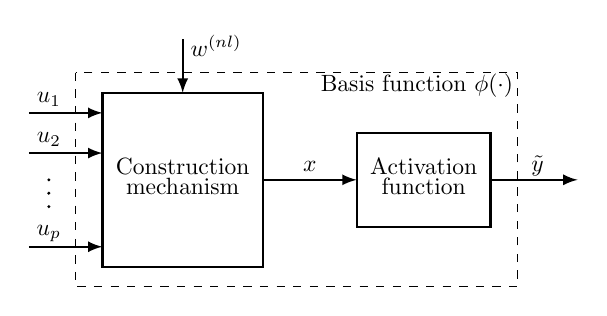
\begin{tikzpicture}[scale=0.85,transform shape]



\draw [thick] (-4.3,3.2) rectangle (-1.9,0.6);
\node at (-3.1,2.1) {Construction};
\node at (-3.1,1.8) {mechanism};
\node at (0.5,2.1) {Activation};
\node at (0.5,1.8) {function};
\draw  [thick] (-0.5,2.6) rectangle (1.5,1.2);
\draw  [thick][-latex](-1.9,1.9) -- (-0.5,1.9);
\node at (-1.2,2.1) {$x$};
\draw [thick] [-latex](1.5,1.9) -- (2.8,1.9);
\node at (2.2,2.1) {$\tilde{y}$};
\draw  [thick][-latex](-5.4,2.9) -- (-4.3,2.9);
\draw  [thick][-latex](-5.4,2.3) -- (-4.3,2.3);
\draw  [thick][-latex](-5.4,0.9) -- (-4.3,0.9);
\node at (-5.1,3.1) {$u_1$};
\node at (-5.1,2.5) {$u_2$};
\node at (-5.1,1.1) {$u_p$};

\node[circle,fill,inner sep=0.5pt] (A) at (-5.1,1.9) {};
\node[circle,fill,inner sep=0.5pt] (A) at (-5.1,1.7) {};
\node[circle,fill,inner sep=0.5pt] (A) at (-5.1,1.5) {};
\draw  [thick][-latex](-3.1,4) -- (-3.1,3.2);
\node at (-2.6,3.9) {$w^{(nl)}$};
\draw [dashed] (-4.7,3.5) rectangle (1.9,0.3);
\node at (0.4,3.3) {Basis function $\phi(\cdot)$};
\end{tikzpicture} 
\caption{Operation of construction mechanism.}
\label{fig:activation_mechanism}
\end{figure}

\vspace{-3mm}

The basis function of the neurons is based on the construction mechanism, that maps the inputs to a scalar $x$ with the help of some non-linear parameters. The activation function then non-linearly transforms the scalar $x$ to the neuron output $\tilde{y}$. 

\subsection{Radial construction}
\label{radial construction}

Among several construction mechanism, the radial construction is further discussed. In this approach the scalar $x$ is calculated as the distance between the inputs and the center of the basis functions such that 

 \begin{equation}
\label{radial_structure}
x = ||u- \mu|| = \sqrt{(u-\mu)^T (u-\mu)},
\end{equation}

where $\mu = (\mu_1 \ \mu_2 \ ... \ \mu_p)^T$ is the center vector of the basis functions. The radial construction is utilized for Radial Basis Function(RBF) networks, which is discussed in the following sections.


\section{RBF networks}
\label{Radial_basis_function_networks}

 In RBF networks, the first task is to calculate the Euclidean norm, i.e. the distance of the input and center vectors. This is the radial construction mechanism, which is shown in \figref{fig:activation_mechanism}. In the second part, this distance $x$ is transformed by the activation function. Therefore, an RBF network is a class of single hidden layer feedforward networks, expressed as the linear combination of radially symmetric non-linear basis functions \cite{RBF_article}. Typically the choice for the basis functions is the Gaussian function, which is formulated in \eqref{Gaussian_activation} 

\begin{equation}
\label{Gaussian_activation}
g(x) = exp \Big(-\frac{1}{2}x^2\Big).
\end{equation}

Substituting the distance $x$ into \eqref{Gaussian_activation}, one RBF neuron can be given such that

 \begin{equation}
\label{Gaussian_activation1}
\phi(u,\mu_k, \psi_k) = exp \Big(-\frac{||u-\mu_k||^2}{2\psi_k^2}\Big), 
\end{equation}

where $\mu_k \in \: \mathbb{R}^{M}$ determines the center of the RBFs, $\psi_k \in \: \mathbb{R}^{M}$ is the standard deviation of the Gaussian, i.e the width parameter and $||\cdot||$ is the Euclidean norm. In a NN, RBFs overlap each other to capture the information from the input data, and the width parameters $\psi_k$ control the amount of these overlapping basis functions. An example is shown in \figref{fig:rbf_pram}, where the influence of these parameters is illustrated on one RBF neuron, with a single input $u$. 

 %RBFs with different parameters
\begin{figure}[H]
\centering
%
\includegraphics[width=0.35\textwidth]{report/pictures/missingfigure}
% This file was created by matlab2tikz.
%
%The latest updates can be retrieved from
%  http://www.mathworks.com/matlabcentral/fileexchange/22022-matlab2tikz-matlab2tikz
%where you can also make suggestions and rate matlab2tikz.
%
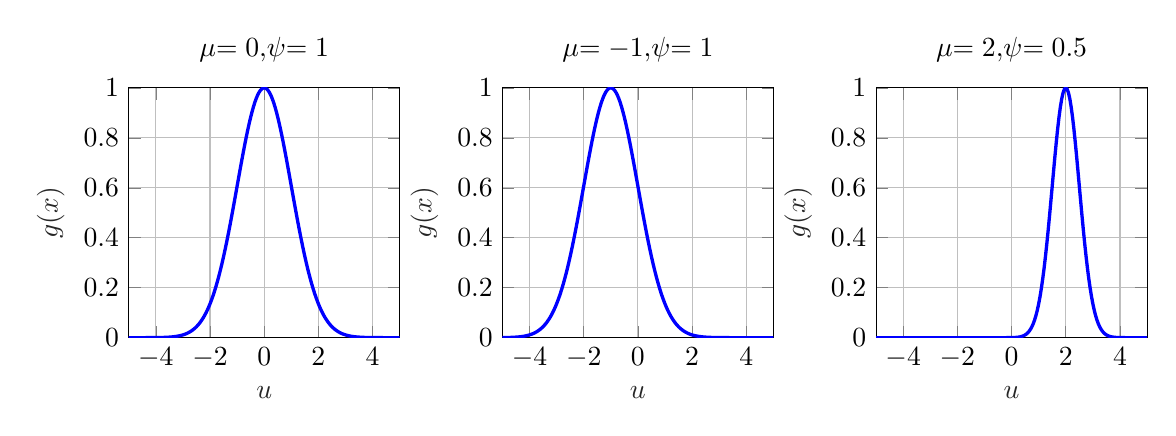
\begin{tikzpicture}

\begin{axis}[%
width=1.355in,
height=1.249in,
at={(1.067in,0.455in)},
scale only axis,
xmin=-5,
xmax=5,
xlabel style={font=\color{white!15!black}},
xlabel={$u$},
ymin=0,
ymax=1,
ylabel style={font=\color{white!15!black}},
ylabel={$g(x)$},
axis background/.style={fill=white},
title style={font=\bfseries},
title={$\mu\text{ = 0, }\psi\text{ = 1}$},
xmajorgrids,
ymajorgrids
]
\addplot [color=blue, line width=1.2pt, forget plot]
  table[row sep=crcr]{%
-5	3.72665317207867e-06\\
-4.95	4.77913973220464e-06\\
-4.9	6.11356796637139e-06\\
-4.85	7.80106730231083e-06\\
-4.8	9.92950430585105e-06\\
-4.75	1.26071051770485e-05\\
-4.7	1.59667838978047e-05\\
-4.65	2.0171295076558e-05\\
-4.6	2.54193465161991e-05\\
-4.55	3.19528237744228e-05\\
-4.5	4.00652973929507e-05\\
-4.45	5.01120028862472e-05\\
-4.4	6.25215037748197e-05\\
-4.35	7.78092686155368e-05\\
-4.3	9.6593413722183e-05\\
-4.25	0.000119612883581023\\
-4.2	0.000147748360232032\\
-4.15	0.000182046210367004\\
-4.1	0.000223745793720617\\
-4.05	0.000274310467493397\\
-4	0.000335462627902507\\
-3.95	0.000409223130228173\\
-3.9	0.000497955421503266\\
-3.85	0.000604414703759546\\
-3.8	0.00073180241888046\\
-3.75	0.000883826306935035\\
-3.7	0.0010647662366679\\
-3.65	0.0012795459378999\\
-3.6	0.00153381067932444\\
-3.55	0.00183401083007313\\
-3.5	0.00218749111818284\\
-3.45	0.00260258525272535\\
-3.4	0.00308871540823671\\
-3.35	0.00365649588005282\\
-3.3	0.00431784000763299\\
-3.25	0.0050860692310126\\
-3.2	0.00597602289500582\\
-3.15	0.00700416714936227\\
-3.1	0.00818870101437391\\
-3.05	0.0095496573950201\\
-3	0.0111089965382421\\
-2.95	0.0128906891440012\\
-2.9	0.0149207860690675\\
-2.85	0.0172274713116347\\
-2.8	0.0198410947443699\\
-2.75	0.0227941808836118\\
-2.7	0.0261214098539177\\
-2.65	0.0298595666411149\\
-2.6	0.0340474547345986\\
-2.55	0.0387257703516635\\
-2.5	0.0439369336234064\\
-2.45	0.0497248734123485\\
-2.4	0.0561347628341325\\
-2.35	0.0632127030752875\\
-2.3	0.0710053537396354\\
-2.25	0.0795595087182259\\
-2.2	0.0889216174593844\\
-2.15	0.0991372525107452\\
-2.1	0.110250525304483\\
-2.05	0.122303453346898\\
-2	0.13533528323661\\
-1.95	0.149381775250415\\
-1.9	0.164474456577152\\
-1.85	0.18063985161889\\
-1.8	0.197898699083611\\
-1.75	0.216265166829883\\
-1.7	0.235746076555859\\
-1.65	0.256340151415069\\
-1.6	0.27803730045319\\
-1.55	0.300817954357271\\
-1.5	0.324652467358345\\
-1.45	0.349500600199751\\
-1.4	0.375311098851394\\
-1.35	0.402021383094649\\
-1.3	0.429557358210734\\
-1.25	0.457833361771608\\
-1.2	0.486752255959966\\
-1.15	0.51620567394549\\
-1.1	0.546074426639704\\
-1.05	0.576229073671794\\
-1	0.606530659712628\\
-0.95	0.636831614371737\\
-0.899999999999999	0.666976810858469\\
-0.85	0.696804775496029\\
-0.8	0.726149037073685\\
-0.75	0.754839601989002\\
-0.7	0.782704538241863\\
-0.649999999999999	0.809571648667882\\
-0.6	0.835270211411267\\
-0.55	0.859632763602538\\
-0.5	0.882496902584591\\
-0.45	0.903707077873192\\
-0.399999999999999	0.923116346386632\\
-0.35	0.940588063364339\\
-0.3	0.955997481833097\\
-0.25	0.969233234476342\\
-0.199999999999999	0.980198673306753\\
-0.149999999999999	0.988813044611232\\
-0.0999999999999996	0.995012479192681\\
-0.0499999999999998	0.99875078092458\\
0	1\\
0.0499999999999998	0.998750780924581\\
0.0999999999999996	0.995012479192683\\
0.149999999999999	0.988813044611234\\
0.199999999999999	0.980198673306757\\
0.25	0.969233234476346\\
0.3	0.955997481833103\\
0.35	0.940588063364345\\
0.399999999999999	0.923116346386639\\
0.45	0.9037070778732\\
0.5	0.8824969025846\\
0.55	0.859632763602547\\
0.6	0.835270211411277\\
0.649999999999999	0.809571648667892\\
0.7	0.782704538241873\\
0.75	0.754839601989013\\
0.8	0.726149037073696\\
0.85	0.69680477549604\\
0.899999999999999	0.66697681085848\\
0.95	0.636831614371749\\
1	0.606530659712639\\
1.05	0.576229073671805\\
1.1	0.546074426639715\\
1.15	0.516205673945502\\
1.2	0.486752255959977\\
1.25	0.457833361771619\\
1.3	0.429557358210744\\
1.35	0.40202138309466\\
1.4	0.375311098851404\\
1.45	0.349500600199761\\
1.5	0.324652467358354\\
1.55	0.30081795435728\\
1.6	0.278037300453198\\
1.65	0.256340151415077\\
1.7	0.235746076555867\\
1.75	0.21626516682989\\
1.8	0.197898699083618\\
1.85	0.180639851618897\\
1.9	0.164474456577157\\
1.95	0.14938177525042\\
2	0.135335283236615\\
2.05	0.122303453346903\\
2.1	0.110250525304487\\
2.15	0.0991372525107492\\
2.2	0.088921617459388\\
2.25	0.0795595087182293\\
2.3	0.0710053537396385\\
2.35	0.0632127030752902\\
2.4	0.056134762834135\\
2.45	0.0497248734123508\\
2.5	0.0439369336234085\\
2.55	0.0387257703516653\\
2.6	0.0340474547346002\\
2.65	0.0298595666411163\\
2.7	0.026121409853919\\
2.75	0.022794180883613\\
2.8	0.0198410947443709\\
2.85	0.0172274713116357\\
2.9	0.0149207860690683\\
2.95	0.0128906891440019\\
3	0.0111089965382427\\
3.05	0.00954965739502065\\
3.1	0.00818870101437438\\
3.15	0.00700416714936269\\
3.2	0.00597602289500618\\
3.25	0.0050860692310129\\
3.3	0.00431784000763326\\
3.35	0.00365649588005305\\
3.4	0.00308871540823691\\
3.45	0.00260258525272552\\
3.5	0.00218749111818299\\
3.55	0.00183401083007325\\
3.6	0.00153381067932454\\
3.65	0.00127954593789999\\
3.7	0.00106476623666798\\
3.75	0.000883826306935097\\
3.8	0.000731802418880512\\
3.85	0.000604414703759589\\
3.9	0.000497955421503302\\
3.95	0.000409223130228203\\
4	0.000335462627902532\\
4.05	0.000274310467493418\\
4.1	0.000223745793720634\\
4.15	0.000182046210367018\\
4.2	0.000147748360232044\\
4.25	0.000119612883581032\\
4.3	9.65934137221907e-05\\
4.35	7.78092686155432e-05\\
4.4	6.25215037748248e-05\\
4.45	5.01120028862513e-05\\
4.5	4.00652973929541e-05\\
4.55	3.19528237744255e-05\\
4.6	2.54193465162013e-05\\
4.65	2.01712950765598e-05\\
4.7	1.59667838978061e-05\\
4.75	1.26071051770496e-05\\
4.8	9.92950430585193e-06\\
4.85	7.80106730231153e-06\\
4.9	6.11356796637196e-06\\
4.95	4.77913973220508e-06\\
5	3.72665317207902e-06\\
};
\end{axis}

\begin{axis}[%
xshift=-0.7cm,
width=1.355in,
height=1.249in,
at={(3.211in,0.455in)},
scale only axis,
xmin=-5,
xmax=5,
xlabel style={font=\color{white!15!black}},
xlabel={$u$},
ymin=0,
ymax=1,
ylabel style={font=\color{white!15!black}},
ylabel={$g(x)$},
axis background/.style={fill=white},
title style={font=\bfseries},
title={$\mu\text{ = -1, }\psi\text{ = 1}$},
xmajorgrids,
ymajorgrids
]
\addplot [color=blue, line width=1.2pt, forget plot]
  table[row sep=crcr]{%
-5	0.000335462627902512\\
-4.95	0.000409223130228179\\
-4.9	0.000497955421503273\\
-4.85	0.000604414703759554\\
-4.8	0.000731802418880471\\
-4.75	0.000883826306935047\\
-4.7	0.00106476623666792\\
-4.65	0.00127954593789992\\
-4.6	0.00153381067932446\\
-4.55	0.00183401083007315\\
-4.5	0.00218749111818287\\
-4.45	0.00260258525272538\\
-4.4	0.00308871540823675\\
-4.35	0.00365649588005287\\
-4.3	0.00431784000763304\\
-4.25	0.00508606923101266\\
-4.2	0.00597602289500589\\
-4.15	0.00700416714936235\\
-4.1	0.008188701014374\\
-4.05	0.00954965739502021\\
-4	0.0111089965382422\\
-3.95	0.0128906891440013\\
-3.9	0.0149207860690677\\
-3.85	0.0172274713116349\\
-3.8	0.01984109474437\\
-3.75	0.0227941808836121\\
-3.7	0.0261214098539179\\
-3.65	0.0298595666411151\\
-3.6	0.0340474547345989\\
-3.55	0.0387257703516639\\
-3.5	0.0439369336234068\\
-3.45	0.0497248734123489\\
-3.4	0.056134762834133\\
-3.35	0.063212703075288\\
-3.3	0.071005353739636\\
-3.25	0.0795595087182265\\
-3.2	0.0889216174593851\\
-3.15	0.099137252510746\\
-3.1	0.110250525304484\\
-3.05	0.122303453346899\\
-3	0.135335283236611\\
-2.95	0.149381775250416\\
-2.9	0.164474456577153\\
-2.85	0.180639851618891\\
-2.8	0.197898699083612\\
-2.75	0.216265166829884\\
-2.7	0.23574607655586\\
-2.65	0.25634015141507\\
-2.6	0.27803730045319\\
-2.55	0.300817954357271\\
-2.5	0.324652467358345\\
-2.45	0.349500600199752\\
-2.4	0.375311098851395\\
-2.35	0.40202138309465\\
-2.3	0.429557358210734\\
-2.25	0.457833361771609\\
-2.2	0.486752255959966\\
-2.15	0.51620567394549\\
-2.1	0.546074426639703\\
-2.05	0.576229073671794\\
-2	0.606530659712627\\
-1.95	0.636831614371737\\
-1.9	0.666976810858468\\
-1.85	0.696804775496028\\
-1.8	0.726149037073685\\
-1.75	0.754839601989001\\
-1.7	0.782704538241862\\
-1.65	0.809571648667881\\
-1.6	0.835270211411267\\
-1.55	0.859632763602537\\
-1.5	0.882496902584591\\
-1.45	0.903707077873192\\
-1.4	0.923116346386632\\
-1.35	0.940588063364339\\
-1.3	0.955997481833097\\
-1.25	0.969233234476342\\
-1.2	0.980198673306753\\
-1.15	0.988813044611232\\
-1.1	0.995012479192681\\
-1.05	0.99875078092458\\
-1	1\\
-0.95	0.998750780924581\\
-0.899999999999999	0.995012479192683\\
-0.85	0.988813044611234\\
-0.8	0.980198673306757\\
-0.75	0.969233234476346\\
-0.7	0.955997481833103\\
-0.649999999999999	0.940588063364345\\
-0.6	0.923116346386639\\
-0.55	0.9037070778732\\
-0.5	0.8824969025846\\
-0.45	0.859632763602547\\
-0.399999999999999	0.835270211411277\\
-0.35	0.809571648667892\\
-0.3	0.782704538241873\\
-0.25	0.754839601989013\\
-0.199999999999999	0.726149037073696\\
-0.149999999999999	0.69680477549604\\
-0.0999999999999996	0.66697681085848\\
-0.0499999999999998	0.636831614371749\\
0	0.606530659712639\\
0.0499999999999998	0.576229073671806\\
0.0999999999999996	0.546074426639715\\
0.149999999999999	0.516205673945502\\
0.199999999999999	0.486752255959977\\
0.25	0.45783336177162\\
0.3	0.429557358210744\\
0.35	0.40202138309466\\
0.399999999999999	0.375311098851405\\
0.45	0.349500600199761\\
0.5	0.324652467358354\\
0.55	0.30081795435728\\
0.6	0.278037300453198\\
0.649999999999999	0.256340151415078\\
0.7	0.235746076555867\\
0.75	0.216265166829891\\
0.8	0.197898699083618\\
0.85	0.180639851618897\\
0.899999999999999	0.164474456577158\\
0.95	0.149381775250421\\
1	0.135335283236615\\
1.05	0.122303453346903\\
1.1	0.110250525304487\\
1.15	0.0991372525107493\\
1.2	0.088921617459388\\
1.25	0.0795595087182293\\
1.3	0.0710053537396385\\
1.35	0.0632127030752901\\
1.4	0.0561347628341349\\
1.45	0.0497248734123507\\
1.5	0.0439369336234084\\
1.55	0.0387257703516652\\
1.6	0.0340474547346001\\
1.65	0.0298595666411162\\
1.7	0.0261214098539189\\
1.75	0.0227941808836129\\
1.8	0.0198410947443707\\
1.85	0.0172274713116355\\
1.9	0.0149207860690682\\
1.95	0.0128906891440018\\
2	0.0111089965382426\\
2.05	0.00954965739502055\\
2.1	0.00818870101437429\\
2.15	0.00700416714936261\\
2.2	0.00597602289500611\\
2.25	0.00508606923101284\\
2.3	0.00431784000763321\\
2.35	0.00365649588005301\\
2.4	0.00308871540823687\\
2.45	0.00260258525272549\\
2.5	0.00218749111818296\\
2.55	0.00183401083007322\\
2.6	0.00153381067932452\\
2.65	0.00127954593789997\\
2.7	0.00106476623666796\\
2.75	0.000883826306935085\\
2.8	0.000731802418880503\\
2.85	0.000604414703759581\\
2.9	0.000497955421503296\\
2.95	0.000409223130228197\\
3	0.000335462627902527\\
3.05	0.000274310467493414\\
3.1	0.000223745793720631\\
3.15	0.000182046210367015\\
3.2	0.000147748360232041\\
3.25	0.000119612883581031\\
3.3	9.65934137221892e-05\\
3.35	7.78092686155419e-05\\
3.4	6.25215037748238e-05\\
3.45	5.01120028862505e-05\\
3.5	4.00652973929535e-05\\
3.55	3.1952823774425e-05\\
3.6	2.54193465162008e-05\\
3.65	2.01712950765595e-05\\
3.7	1.59667838978058e-05\\
3.75	1.26071051770494e-05\\
3.8	9.92950430585177e-06\\
3.85	7.80106730231139e-06\\
3.9	6.11356796637185e-06\\
3.95	4.77913973220499e-06\\
4	3.72665317207895e-06\\
4.05	2.89869477463316e-06\\
4.1	2.24905596703252e-06\\
4.15	1.74065339649344e-06\\
4.2	1.34381227763163e-06\\
4.25	1.03485421110946e-06\\
4.3	7.94939361534982e-07\\
4.35	6.09120331551606e-07\\
4.4	4.6557157157835e-07\\
4.45	3.54963808697164e-07\\
4.5	2.69957850336326e-07\\
4.55	2.04796302119765e-07\\
4.6	1.54975313570305e-07\\
4.65	1.1698150401353e-07\\
4.7	8.80817919646143e-08\\
4.75	6.61560163769838e-08\\
4.8	4.95640531917301e-08\\
4.85	3.70406455079473e-08\\
4.9	2.76124245682834e-08\\
4.95	2.05326404492339e-08\\
5	1.52299797447143e-08\\
};
\end{axis}

\begin{axis}[%
xshift=-1.4cm,
width=1.355in,
height=1.249in,
at={(5.355in,0.455in)},
scale only axis,
xmin=-5,
xmax=5,
xlabel style={font=\color{white!15!black}},
xlabel={$u$},
ymin=0,
ymax=1,
ylabel style={font=\color{white!15!black}},
ylabel={$g(x)$},
axis background/.style={fill=white},
title style={font=\bfseries},
title={$\mu\text{ = 2, }\psi\text{ = 0.5}$},
xmajorgrids,
ymajorgrids
]
\addplot [color=blue, line width=1.2pt, forget plot]
  table[row sep=crcr]{%
-5	2.74878500791021e-43\\
-4.95	1.10912776125503e-42\\
-4.9	4.43077231241282e-42\\
-4.85	1.75240444373849e-41\\
-4.8	6.86193047676127e-41\\
-4.75	2.66020641594391e-40\\
-4.7	1.02103684608935e-39\\
-4.65	3.87993587628423e-39\\
-4.6	1.45970379320953e-38\\
-4.55	5.43703314193213e-38\\
-4.5	2.00500878196157e-37\\
-4.45	7.32027899105949e-37\\
-4.4	2.64603779068747e-36\\
-4.35	9.46937917271538e-36\\
-4.3	3.35508885623091e-35\\
-4.25	1.17691094392159e-34\\
-4.2	4.08733497286565e-34\\
-4.15	1.40538047776279e-33\\
-4.1	4.7841485558165e-33\\
-4.05	1.6123987480501e-32\\
-4	5.38018616002068e-32\\
-3.95	1.77737557956817e-31\\
-3.9	5.81323888488905e-31\\
-3.85	1.88240984759479e-30\\
-3.8	6.03486080597041e-30\\
-3.75	1.91547895196696e-29\\
-3.7	6.01928027681589e-29\\
-3.65	1.87270255445602e-28\\
-3.6	5.76832996124723e-28\\
-3.55	1.75909154968455e-27\\
-3.5	5.31109224967845e-27\\
-3.45	1.58758249826435e-26\\
-3.4	4.69835486089745e-26\\
-3.35	1.37661463866175e-25\\
-3.3	3.99333740985715e-25\\
-3.25	1.14687658222545e-24\\
-3.2	3.26102718071061e-24\\
-3.15	9.18013795095797e-24\\
-3.1	2.55859208104832e-23\\
-3.05	7.06008533726155e-23\\
-3	1.92874984796364e-22\\
-2.95	5.2167366620263e-22\\
-2.9	1.3969439431469e-21\\
-2.85	3.70353197765179e-21\\
-2.8	9.72098502029933e-21\\
-2.75	2.52616378092532e-20\\
-2.7	6.49934797206988e-20\\
-2.65	1.65552266209852e-19\\
-2.6	4.17501005584986e-19\\
-2.55	1.04240617839e-18\\
-2.5	2.57675710915456e-18\\
-2.45	6.30618989398542e-18\\
-2.4	1.52797996828705e-17\\
-2.35	3.66543339560045e-17\\
-2.3	8.70542662229477e-17\\
-2.25	2.04697171316387e-16\\
-2.2	4.76530473529831e-16\\
-2.15	1.09831412982841e-15\\
-2.1	2.50622188714485e-15\\
-2.05	5.66199551694798e-15\\
-2	1.2664165549092e-14\\
-1.95	2.80440473822231e-14\\
-1.9	6.14839641270375e-14\\
-1.85	1.33456608482178e-13\\
-1.8	2.86797500888764e-13\\
-1.75	6.10193667760435e-13\\
-1.7	1.28533722513345e-12\\
-1.65	2.68054763731221e-12\\
-1.6	5.53461007170021e-12\\
-1.55	1.13137762000636e-11\\
-1.5	2.28973484564523e-11\\
-1.45	4.58796248713866e-11\\
-1.4	9.10147076448671e-11\\
-1.35	1.78755887112773e-10\\
-1.3	3.47589128123947e-10\\
-1.25	6.69158609129193e-10\\
-1.2	1.27540762952588e-09\\
-1.15	2.40672243630074e-09\\
-1.1	4.49634946228031e-09\\
-1.05	8.31670245682736e-09\\
-1	1.52299797447108e-08\\
-0.95	2.76124245682771e-08\\
-0.899999999999999	4.95640531917193e-08\\
-0.85	8.80817919645962e-08\\
-0.8	1.54975313570273e-07\\
-0.75	2.69957850336272e-07\\
-0.7	4.65571571578261e-07\\
-0.649999999999999	7.94939361534836e-07\\
-0.6	1.34381227763139e-06\\
-0.55	2.24905596703212e-06\\
-0.5	3.72665317207832e-06\\
-0.45	6.11356796637084e-06\\
-0.399999999999999	9.9295043058502e-06\\
-0.35	1.59667838978033e-05\\
-0.3	2.5419346516197e-05\\
-0.25	4.00652973929477e-05\\
-0.199999999999999	6.2521503774815e-05\\
-0.149999999999999	9.65934137221763e-05\\
-0.0999999999999996	0.000147748360232022\\
-0.0499999999999998	0.000223745793720603\\
0	0.000335462627902487\\
0.0499999999999998	0.000497955421503237\\
0.0999999999999996	0.00073180241888042\\
0.149999999999999	0.00106476623666785\\
0.199999999999999	0.00153381067932436\\
0.25	0.00218749111818274\\
0.3	0.00308871540823657\\
0.35	0.00431784000763281\\
0.399999999999999	0.00597602289500558\\
0.45	0.0081887010143736\\
0.5	0.0111089965382417\\
0.55	0.014920786069067\\
0.6	0.0198410947443693\\
0.649999999999999	0.0261214098539169\\
0.7	0.0340474547345977\\
0.75	0.0439369336234054\\
0.8	0.0561347628341313\\
0.85	0.0710053537396339\\
0.899999999999999	0.0889216174593828\\
0.95	0.110250525304481\\
1	0.135335283236608\\
1.05	0.164474456577149\\
1.1	0.197898699083608\\
1.15	0.235746076555856\\
1.2	0.278037300453186\\
1.25	0.324652467358341\\
1.3	0.37531109885139\\
1.35	0.429557358210729\\
1.4	0.486752255959961\\
1.45	0.546074426639699\\
1.5	0.606530659712623\\
1.55	0.666976810858464\\
1.6	0.726149037073681\\
1.65	0.782704538241859\\
1.7	0.835270211411264\\
1.75	0.882496902584588\\
1.8	0.92311634638663\\
1.85	0.955997481833095\\
1.9	0.980198673306752\\
1.95	0.995012479192681\\
2	1\\
2.05	0.995012479192684\\
2.1	0.980198673306759\\
2.15	0.955997481833105\\
2.2	0.923116346386642\\
2.25	0.882496902584603\\
2.3	0.835270211411281\\
2.35	0.782704538241878\\
2.4	0.726149037073702\\
2.45	0.666976810858486\\
2.5	0.606530659712645\\
2.55	0.546074426639721\\
2.6	0.486752255959984\\
2.65	0.429557358210751\\
2.7	0.375311098851411\\
2.75	0.32465246735836\\
2.8	0.278037300453204\\
2.85	0.235746076555872\\
2.9	0.197898699083623\\
2.95	0.164474456577162\\
3	0.135335283236619\\
3.05	0.110250525304491\\
3.1	0.088921617459391\\
3.15	0.0710053537396409\\
3.2	0.056134762834137\\
3.25	0.0439369336234101\\
3.3	0.0340474547346016\\
3.35	0.02612140985392\\
3.4	0.0198410947443717\\
3.45	0.014920786069069\\
3.5	0.0111089965382432\\
3.55	0.00818870101437477\\
3.6	0.00597602289500647\\
3.65	0.00431784000763347\\
3.7	0.00308871540823707\\
3.75	0.0021874911181831\\
3.8	0.00153381067932462\\
3.85	0.00106476623666804\\
3.9	0.000731802418880555\\
3.95	0.000497955421503332\\
4	0.000335462627902552\\
4.05	0.000223745793720648\\
4.1	0.000147748360232053\\
4.15	9.65934137221969e-05\\
4.2	6.25215037748289e-05\\
4.25	4.00652973929568e-05\\
4.3	2.5419346516203e-05\\
4.35	1.59667838978072e-05\\
4.4	9.92950430585265e-06\\
4.45	6.11356796637241e-06\\
4.5	3.7266531720793e-06\\
4.55	2.24905596703273e-06\\
4.6	1.34381227763176e-06\\
4.65	7.94939361535061e-07\\
4.7	4.65571571578397e-07\\
4.75	2.69957850336354e-07\\
4.8	1.54975313570321e-07\\
4.85	8.80817919646237e-08\\
4.9	4.95640531917355e-08\\
4.95	2.76124245682864e-08\\
5	1.5229979744716e-08\\
};
\end{axis}
\end{tikzpicture}% 
\caption{The width and the position of the Gaussian activation function in terms of $\psi$ and $\mu$.}
\label{fig:rbf_pram}
\end{figure}

\vspace{-3mm}

Therefore, when an RBF network is chosen for identification, three types of parameters need to be considered. The output weights $w_i$ are linear parameters. They define the heights of the basis functions and the bias, i.e the offset value. The centers $\mu$ are non-linear parameters of the hidden layer neurons. They determine the positions of the basis functions. Furthermore, the standard deviations $\psi$ are also non-linear parameters of the hidden-layer neurons. During the optimization, these parameters have to be somehow determined and optimized. As it was mentioned in \secref{neural_networks}, the linear parameters are going to be optimized, while the non-linear properties of the RBFs is going to be determined with some technique, described in the following. 

\figref{fig:rbf_interpol} illustrates the interpolation and extrapolation capability of the RBF networks. 

 %Interpolation of RBFS
\begin{figure}[H]
\centering
%
\includegraphics[width=0.35\textwidth]{report/pictures/missingfigure}
% This file was created by matlab2tikz.
%
%The latest updates can be retrieved from
%  http://www.mathworks.com/matlabcentral/fileexchange/22022-matlab2tikz-matlab2tikz
%where you can also make suggestions and rate matlab2tikz.
%
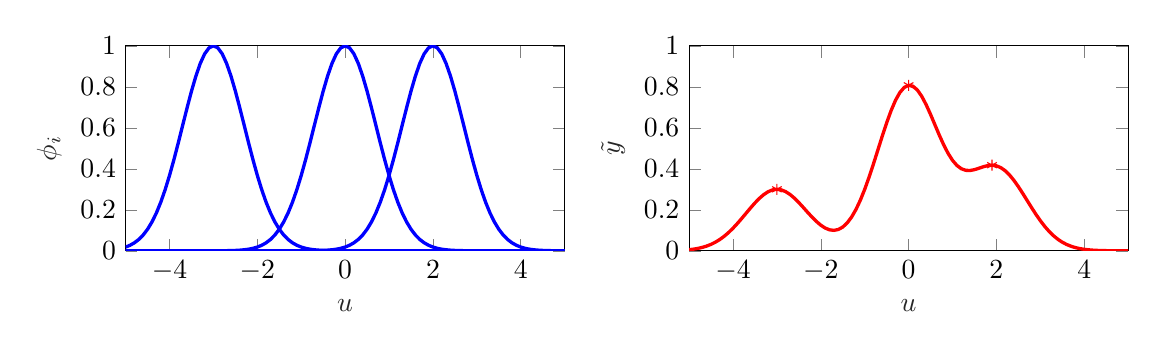
\begin{tikzpicture}

\begin{axis}[%
width=2.195in,
height=1.025in,
at={(0.93in,0.43in)},
scale only axis,
xmin=-5,
xmax=5,
xlabel style={font=\color{white!15!black}},
xlabel={$u$},
ymin=0,
ymax=1,
ylabel style={font=\color{white!15!black}},
ylabel={$\phi{}_\text{i}$},
axis background/.style={fill=white}
]
\addplot [color=blue, line width=1.2pt, forget plot]
  table[row sep=crcr]{%
-5	1.3887943864964e-11\\
-4.9	3.73757132794424e-11\\
-4.8	9.85950557599152e-11\\
-4.7	2.54938188039196e-10\\
-4.6	6.46143177310613e-10\\
-4.5	1.60522805518561e-09\\
-4.4	3.90893843426485e-09\\
-4.3	9.33028757450501e-09\\
-4.2	2.18295779512548e-08\\
-4.1	5.00621802076705e-08\\
-4	1.12535174719259e-07\\
-3.9	2.47959601804503e-07\\
-3.8	5.35534780279311e-07\\
-3.7	1.13372713874796e-06\\
-3.6	2.35257520000978e-06\\
-3.5	4.78511739212901e-06\\
-3.4	9.54016287307925e-06\\
-3.3	1.86437423315169e-05\\
-3.2	3.57128496416351e-05\\
-3.1	6.70548243028112e-05\\
-3	0.00012340980408668\\
-2.9	0.000222629856918889\\
-2.8	0.000393669040655079\\
-2.7	0.000682328052756378\\
-2.6	0.00115922917390459\\
-2.5	0.00193045413622771\\
-2.4	0.00315111159844444\\
-2.3	0.00504176025969098\\
-2.2	0.00790705405159345\\
-2.1	0.012155178329915\\
-2	0.0183156388887342\\
-1.9	0.0270518468663504\\
-1.8	0.0391638950989871\\
-1.7	0.0555762126114831\\
-1.6	0.0773047404432999\\
-1.5	0.105399224561864\\
-1.4	0.140858420921045\\
-1.3	0.184519523992989\\
-1.2	0.236927758682122\\
-1.1	0.298197279429888\\
-1	0.367879441171442\\
-0.899999999999999	0.444858066222942\\
-0.8	0.527292424043049\\
-0.7	0.612626394184416\\
-0.6	0.697676326071031\\
-0.5	0.778800783071405\\
-0.399999999999999	0.852143788966212\\
-0.3	0.913931185271228\\
-0.199999999999999	0.960789439152324\\
-0.0999999999999996	0.990049833749168\\
0	1\\
0.0999999999999996	0.990049833749168\\
0.199999999999999	0.960789439152324\\
0.3	0.913931185271228\\
0.399999999999999	0.852143788966212\\
0.5	0.778800783071405\\
0.6	0.697676326071031\\
0.7	0.612626394184416\\
0.8	0.527292424043049\\
0.899999999999999	0.444858066222942\\
1	0.367879441171442\\
1.1	0.298197279429888\\
1.2	0.236927758682122\\
1.3	0.184519523992989\\
1.4	0.140858420921045\\
1.5	0.105399224561864\\
1.6	0.0773047404432999\\
1.7	0.0555762126114831\\
1.8	0.0391638950989871\\
1.9	0.0270518468663504\\
2	0.0183156388887342\\
2.1	0.012155178329915\\
2.2	0.00790705405159345\\
2.3	0.00504176025969098\\
2.4	0.00315111159844444\\
2.5	0.00193045413622771\\
2.6	0.00115922917390459\\
2.7	0.000682328052756378\\
2.8	0.000393669040655079\\
2.9	0.000222629856918889\\
3	0.00012340980408668\\
3.1	6.70548243028112e-05\\
3.2	3.57128496416351e-05\\
3.3	1.86437423315169e-05\\
3.4	9.54016287307925e-06\\
3.5	4.78511739212901e-06\\
3.6	2.35257520000978e-06\\
3.7	1.13372713874796e-06\\
3.8	5.35534780279311e-07\\
3.9	2.47959601804503e-07\\
4	1.12535174719259e-07\\
4.1	5.00621802076705e-08\\
4.2	2.18295779512548e-08\\
4.3	9.33028757450501e-09\\
4.4	3.90893843426485e-09\\
4.5	1.60522805518561e-09\\
4.6	6.46143177310613e-10\\
4.7	2.54938188039196e-10\\
4.8	9.85950557599152e-11\\
4.9	3.73757132794424e-11\\
5	1.3887943864964e-11\\
};
\addplot [color=blue, line width=1.2pt, forget plot]
  table[row sep=crcr]{%
-5	5.24288566336346e-22\\
-4.9	2.10493997833972e-21\\
-4.8	8.28367700768292e-21\\
-4.7	3.19536671774834e-20\\
-4.6	1.20818201989998e-19\\
-4.5	4.4777324417183e-19\\
-4.4	1.62666462145323e-18\\
-4.3	5.79231288539487e-18\\
-4.2	2.02171584869533e-17\\
-4.1	6.91675397554149e-17\\
-4	2.31952283024357e-16\\
-3.9	7.62445990538972e-16\\
-3.8	2.45659536879214e-15\\
-3.7	7.75840207569605e-15\\
-3.6	2.40173478162097e-14\\
-3.5	7.28772409581969e-14\\
-3.4	2.16756888261895e-13\\
-3.3	6.31928588517537e-13\\
-3.2	1.80583143751321e-12\\
-3.1	5.0582527428438e-12\\
-3	1.3887943864964e-11\\
-2.9	3.73757132794424e-11\\
-2.8	9.85950557599152e-11\\
-2.7	2.54938188039199e-10\\
-2.6	6.46143177310613e-10\\
-2.5	1.60522805518561e-09\\
-2.4	3.90893843426485e-09\\
-2.3	9.33028757450501e-09\\
-2.2	2.18295779512549e-08\\
-2.1	5.00621802076705e-08\\
-2	1.12535174719259e-07\\
-1.9	2.47959601804503e-07\\
-1.8	5.35534780279311e-07\\
-1.7	1.13372713874797e-06\\
-1.6	2.35257520000978e-06\\
-1.5	4.78511739212901e-06\\
-1.4	9.54016287307925e-06\\
-1.3	1.86437423315169e-05\\
-1.2	3.57128496416353e-05\\
-1.1	6.70548243028112e-05\\
-1	0.00012340980408668\\
-0.899999999999999	0.00022262985691889\\
-0.8	0.000393669040655079\\
-0.7	0.000682328052756376\\
-0.6	0.00115922917390459\\
-0.5	0.00193045413622771\\
-0.399999999999999	0.00315111159844445\\
-0.3	0.00504176025969098\\
-0.199999999999999	0.00790705405159346\\
-0.0999999999999996	0.012155178329915\\
0	0.0183156388887342\\
0.0999999999999996	0.0270518468663504\\
0.199999999999999	0.039163895098987\\
0.3	0.055576212611483\\
0.399999999999999	0.0773047404432996\\
0.5	0.105399224561864\\
0.6	0.140858420921045\\
0.7	0.184519523992989\\
0.8	0.236927758682122\\
0.899999999999999	0.298197279429887\\
1	0.367879441171442\\
1.1	0.444858066222941\\
1.2	0.527292424043048\\
1.3	0.612626394184416\\
1.4	0.697676326071031\\
1.5	0.778800783071405\\
1.6	0.852143788966211\\
1.7	0.913931185271228\\
1.8	0.960789439152323\\
1.9	0.990049833749168\\
2	1\\
2.1	0.990049833749168\\
2.2	0.960789439152323\\
2.3	0.913931185271228\\
2.4	0.852143788966211\\
2.5	0.778800783071405\\
2.6	0.697676326071031\\
2.7	0.612626394184416\\
2.8	0.527292424043049\\
2.9	0.444858066222941\\
3	0.367879441171442\\
3.1	0.298197279429888\\
3.2	0.236927758682122\\
3.3	0.184519523992989\\
3.4	0.140858420921045\\
3.5	0.105399224561864\\
3.6	0.0773047404432999\\
3.7	0.055576212611483\\
3.8	0.0391638950989871\\
3.9	0.0270518468663504\\
4	0.0183156388887342\\
4.1	0.012155178329915\\
4.2	0.00790705405159343\\
4.3	0.00504176025969098\\
4.4	0.00315111159844444\\
4.5	0.00193045413622771\\
4.6	0.00115922917390459\\
4.7	0.000682328052756376\\
4.8	0.000393669040655079\\
4.9	0.000222629856918889\\
5	0.00012340980408668\\
};
\addplot [color=blue, line width=1.2pt, forget plot]
  table[row sep=crcr]{%
-5	0.0183156388887342\\
-4.9	0.0270518468663504\\
-4.8	0.0391638950989871\\
-4.7	0.055576212611483\\
-4.6	0.0773047404432999\\
-4.5	0.105399224561864\\
-4.4	0.140858420921045\\
-4.3	0.184519523992989\\
-4.2	0.236927758682122\\
-4.1	0.298197279429888\\
-4	0.367879441171442\\
-3.9	0.444858066222941\\
-3.8	0.527292424043049\\
-3.7	0.612626394184416\\
-3.6	0.697676326071031\\
-3.5	0.778800783071405\\
-3.4	0.852143788966211\\
-3.3	0.913931185271228\\
-3.2	0.960789439152323\\
-3.1	0.990049833749168\\
-3	1\\
-2.9	0.990049833749168\\
-2.8	0.960789439152323\\
-2.7	0.913931185271228\\
-2.6	0.852143788966211\\
-2.5	0.778800783071405\\
-2.4	0.697676326071031\\
-2.3	0.612626394184416\\
-2.2	0.527292424043048\\
-2.1	0.444858066222941\\
-2	0.367879441171442\\
-1.9	0.298197279429887\\
-1.8	0.236927758682122\\
-1.7	0.184519523992989\\
-1.6	0.140858420921045\\
-1.5	0.105399224561864\\
-1.4	0.0773047404432997\\
-1.3	0.055576212611483\\
-1.2	0.039163895098987\\
-1.1	0.0270518468663504\\
-1	0.0183156388887342\\
-0.899999999999999	0.0121551783299149\\
-0.8	0.00790705405159343\\
-0.7	0.00504176025969098\\
-0.6	0.00315111159844444\\
-0.5	0.00193045413622771\\
-0.399999999999999	0.00115922917390459\\
-0.3	0.000682328052756376\\
-0.199999999999999	0.000393669040655077\\
-0.0999999999999996	0.000222629856918889\\
0	0.00012340980408668\\
0.0999999999999996	6.70548243028112e-05\\
0.199999999999999	3.57128496416354e-05\\
0.3	1.86437423315169e-05\\
0.399999999999999	9.54016287307926e-06\\
0.5	4.78511739212901e-06\\
0.6	2.35257520000978e-06\\
0.7	1.13372713874796e-06\\
0.8	5.35534780279311e-07\\
0.899999999999999	2.47959601804504e-07\\
1	1.12535174719259e-07\\
1.1	5.00621802076705e-08\\
1.2	2.18295779512549e-08\\
1.3	9.33028757450501e-09\\
1.4	3.90893843426485e-09\\
1.5	1.60522805518561e-09\\
1.6	6.46143177310613e-10\\
1.7	2.54938188039199e-10\\
1.8	9.85950557599152e-11\\
1.9	3.73757132794424e-11\\
2	1.3887943864964e-11\\
2.1	5.0582527428438e-12\\
2.2	1.80583143751323e-12\\
2.3	6.31928588517537e-13\\
2.4	2.16756888261895e-13\\
2.5	7.28772409581969e-14\\
2.6	2.40173478162097e-14\\
2.7	7.75840207569611e-15\\
2.8	2.45659536879214e-15\\
2.9	7.62445990538972e-16\\
3	2.31952283024357e-16\\
3.1	6.91675397554149e-17\\
3.2	2.02171584869533e-17\\
3.3	5.79231288539487e-18\\
3.4	1.62666462145323e-18\\
3.5	4.4777324417183e-19\\
3.6	1.20818201989998e-19\\
3.7	3.19536671774834e-20\\
3.8	8.28367700768292e-21\\
3.9	2.10493997833972e-21\\
4	5.24288566336346e-22\\
4.1	1.28001531905165e-22\\
4.2	3.06319086457743e-23\\
4.3	7.1853356359022e-24\\
4.4	1.65209178231426e-24\\
4.5	3.72336312175051e-25\\
4.6	8.22528065160669e-26\\
4.7	1.78106663475708e-26\\
4.8	3.7802778447761e-27\\
4.9	7.86468593576642e-28\\
5	1.60381089054864e-28\\
};
\end{axis}

\begin{axis}[%
xshift=-0.85cm,
width=2.195in,
height=1.025in,
at={(4.082in,0.43in)},
scale only axis,
xmin=-5,
xmax=5,
xlabel style={font=\color{white!15!black}},
xlabel={$u$},
ymin=0,
ymax=1,
ylabel style={font=\color{white!15!black}},
ylabel={$\tilde{y}$},
axis background/.style={fill=white}
]
\addplot [color=red, line width=1.2pt, forget plot]
  table[row sep=crcr]{%
-5	0.00549469167773061\\
-4.9	0.00811555408980568\\
-4.8	0.0117491686085722\\
-4.7	0.0166728639873955\\
-4.6	0.0231914226499045\\
-4.5	0.0316197686527417\\
-4.4	0.0422575294034642\\
-4.3	0.0553558646621269\\
-4.2	0.0710783450682989\\
-4.1	0.0894592238787105\\
-4	0.110363922379573\\
-3.9	0.133457618234564\\
-3.8	0.15818815564074\\
-3.7	0.183788825237039\\
-3.6	0.209304779881479\\
-3.5	0.233644063015364\\
-3.4	0.255650768820249\\
-3.3	0.274194270575486\\
-3.2	0.288265402026133\\
-3.1	0.297068593986216\\
-3	0.300098727848825\\
-2.9	0.297193054025236\\
-2.8	0.288551767017659\\
-2.7	0.274725218125549\\
-2.6	0.256570520287444\\
-2.5	0.235184598872495\\
-2.4	0.21182378866364\\
-2.3	0.187821330195193\\
-2.2	0.16451337918602\\
-2.1	0.143181582555686\\
-2	0.12501638847649\\
-1.9	0.111100760505887\\
-1.8	0.102409657897738\\
-1.7	0.0998172807779387\\
-1.6	0.104102259661033\\
-1.5	0.115941061065008\\
-1.4	0.135881974934975\\
-1.3	0.164295940474769\\
-1.2	0.20130566061525\\
-1.1	0.246700199533536\\
-1	0.299847608525409\\
-0.899999999999999	0.359622058420095\\
-0.8	0.424363523066179\\
-0.7	0.491886574646543\\
-0.6	0.55955008600592\\
-0.5	0.624391944352483\\
-0.399999999999999	0.683323244564519\\
-0.3	0.733366350736686\\
-0.199999999999999	0.771912473654693\\
-0.0999999999999996	0.796968727288376\\
0	0.80736327849672\\
0.0999999999999996	0.802880722193165\\
0.199999999999999	0.784307823216346\\
0.3	0.753381026384275\\
0.399999999999999	0.712639789399151\\
0.5	0.665201751817087\\
0.6	0.614485134997803\\
0.7	0.56390926506287\\
0.8	0.516605203367722\\
0.899999999999999	0.475165439138189\\
1	0.441455363166283\\
1.1	0.416501065051741\\
1.2	0.40045918311179\\
1.3	0.392666179667244\\
1.4	0.39175726833793\\
1.5	0.395839693359622\\
1.6	0.402701308134967\\
1.7	0.410033444274159\\
1.8	0.415646891769697\\
1.9	0.41766141100396\\
2	0.414652511115154\\
2.1	0.405744076165117\\
2.2	0.390641418902746\\
2.3	0.369605882316434\\
2.4	0.343378404865305\\
2.5	0.313064676537566\\
2.6	0.279997913767543\\
2.7	0.245596420115974\\
2.8	0.211231904849744\\
2.9	0.178121330374712\\
3	0.147250504311846\\
3.1	0.119332555631397\\
3.2	0.094799673752562\\
3.3	0.073822724591061\\
3.4	0.0563510004987165\\
3.5	0.0421635179186594\\
3.6	0.0309237782374799\\
3.7	0.0222313920263042\\
3.8	0.0156659864674191\\
3.9	0.0108209371142216\\
4	0.00732634558363345\\
4.1	0.00486211138171015\\
4.2	0.00316283908429973\\
4.3	0.00201671156810645\\
4.4	0.00126044776652852\\
4.5	0.000772182938673528\\
4.6	0.000463692186476379\\
4.7	0.000272931425053101\\
4.8	0.000157467695138076\\
4.9	8.90519726681261e-05\\
5	4.93639327450269e-05\\
};
\addplot [color=red, dashdotted, mark=asterisk, mark options={solid, red}, forget plot]
  table[row sep=crcr]{%
-3	0.300098727848825\\
};
\addplot [color=red, dashdotted, mark=asterisk, mark options={solid, red}, forget plot]
  table[row sep=crcr]{%
0	0.80736327849672\\
};
\addplot [color=red, dashdotted, mark=asterisk, mark options={solid, red}, forget plot]
  table[row sep=crcr]{%
1.9	0.41766141100396\\
};
\end{axis}
\end{tikzpicture}% 
\caption{Interpolation and extrapolation of an RBF network without offset.}
\label{fig:rbf_interpol}
\end{figure}

\vspace{-3mm}

In \figref{fig:rbf_interpol}, the basis functions are shown on the left, while the network outputs are shown on the right. The network interpolates  between the three data points marked in the output graph on the right. 

\subsection{RBF training}
\label{RBF_training}

The process of estimating the basis functions $\phi_i$ consists of two problems. One task is to determine a set of $M$ RBFs and then the other task is to estimate the optimal output weights $w_i$ and bias parameters $w_0$. Therefore, the RBF network parameters are generally determined in a two-stage procedure, while in other type of networks the parameters are determined simultaneously by non-linear optimization\cite{RBF_article}. As the output layer of RBF networks linearly combines the Gaussian basis functions, most strategies determine the parameters $\mu$ and $\psi$ of the hidden layer, and then the output layer weighs $w$ by using some linear optimization methods, such as Least Squares(LS) methods. This two-step procedure allows to vary only the weights between the hidden and output layer of the network during the training. 

As the first step, the parameters of the Gaussian basis functions, $\mu$ and $\psi$ are discussed and then the calculation of the weight parameters is explained. 

\subsection{Determination of the hidden layer parameters}
\label{determination_hidden_layer}

As discussed in \secref{RBF_training}, the parameters $\mu$ and $\psi$ of the neurons are not determined through optimization. Instead, one approach is to determine these parameters only by using the input data set $u$. The most commonly applied approach for such tasks is the application of clustering techniques \cite{nelles2013nonlinear}. The clustering of the input data allows to determine the center $\mu$ of the basis functions, according to the distribution of the input data set. Thus, many RBFs are placed in regions where data is dense, and few RBFs are placed in regions where data is less dense.  

The most commonly applied clustering technique in RBF networks is the k-means algorithm \cite{nelles2013nonlinear}. A cluster in the input data set can be defined as a group of data that are more similar to each other than data belonging to other clusters. Initially, the values for the $M$ number of center points is chosen\footnote{The $M$ number of center points of the clusters correspond to the number of basis functions, thus the number of neurons.}. This can be done by choosing randomly $M$ different data samples. Then the algorithm assigns all data samples to their nearest cluster center. When the $M$ clusters are separated, a new mean is calculated for each cluster. Each cluster center is set to the mean of its cluster such that

\begin{equation}
\label{cluster_center}
c_k = \frac{1}{N_k} \sum_{i \in \mathcal{A}_k}  u_i,
\end{equation}

where $i$ runs over the $N_k$ data samples that belong to cluster $k$, which are in the set $\mathcal{A}_k$ and $N_k$ is the number of elements in the set $\mathcal{A}_k$. Eventually, the algorithm stops when the center values $c_k$ do not change in the further iteration steps. The $c_k$ center parameters of the clusters then define the centers $\mu_k$ of the activation functions. Therefore, the k-means algorithm determines the centers $\mu$, in an unsupervised manner, meaning that the RBFs are not automatically moving to the regions where they are required for a good approximation of the system. However, if the number of RBF neurons is being sufficient enough, the NN can give a good approximation of the process. Compared to the supervised learning techniques, where the basis function parameters are to be optimized, the increased number of neurons does not cause increased training time, since both the k-means and LS algorithms are very fast \cite{nelles2013nonlinear}. 

After the clustering is completed, and the $c_k$ cluster centers are assigned to the $\mu$ basis function centers, the width parameters $\psi$ can be determined by the k-nearest rule. This method assigns each RBF a width parameter proportional to the average distance between its center and the input data set in the corresponding cluster such that 

 \begin{equation}
\label{cluster center}
\psi^2 = \frac{1}{N_k} \sum_{i \in \mathcal{A}_k}  ||u_i - \mu_k||^2.
\end{equation}

\subsection{Determination of the weights}
\label{determination_weights} 

The determination of the weights $w_i$ is treated as a LS problem. Using the notation of \figref{fig:nonlin_block}, the error between the measured output data $y$ and the output of the model $\tilde{y}$ is used for the following loss function

 \begin{equation}
\label{loss_function}
L(w) = \frac{1}{2} e^Te \ \rightarrow \ \underset{w}{min}. 
\end{equation}

This is the simplest loss function which says that the loss is proportional to the square of the difference between the model and the process output. 

\section{RBFNN model of the Multi-inlet,Multi-WT system}
\label{RBFNN_model_multi_inlet_multi_WT_sys} 

As the tools for identification has been introduced in \secref{neural_networks} , the interpretation of the Multi-inlet, Multi-WT system in the context of NNs is considered. In order to formulate a NN structure, let us first recall the system equations, described in \secref{model_structure_of_the_multi_inlet_multi_WT_system}. The corresponding output and state equations are shown in \eqref{identification_model11}. 

\begin{equation}
\begin{cases}
  \label{identification_model11}
    \tilde{y}  = \tilde{f}_1(\bar{d}_{\mathcal{K}}, \sigma, \hat{h}_t )\\
  \hat{p}_{k+1} = \tilde{f}_2(\bar{d}_{\mathcal{K},k}, \sigma_k) + a_1 \hat{p}_k + a_2 \hat{h} .
  \end{cases}
\end{equation} 

As it was concluded, the output is governed by the non-linear function $\tilde{f}_1$, which maps the inputs $\bar{d}_{\mathcal{K}}$, $\sigma$ and $\hat{h}_t $ to the outputs $\tilde{y}$. This static input-output system can be represented with a RBFNN, shown in \figref{fig:nn_output}.

  %NN model of the output eq.
 \begin{figure}[H]
 \centering
 %
\includegraphics[width=0.35\textwidth]{report/pictures/missingfigure}
 \begin{tikzpicture}[
scale = 1,
plain/.style={
  draw=none,
  fill=none,
  },
net1/.style={
  matrix of nodes,
  nodes={
    draw,
    circle,
    thick,
    inner sep=8pt
    },
  nodes in empty cells,
  column sep=1.75cm,
  row sep=-11.5pt
  },
>=latex
]

\matrix[net1] (mat)
{
  &  & |[plain]|  \\
 |[plain]| & |[plain]|  \\
|[plain]| & |[plain]|  &  |[plain]|\\
 |[plain]| & |[plain]|  \\
 &   & \\
|[plain]| & |[plain]| &  |[plain]|\\
|[plain]| & |[plain]|   & |[plain]|\\
|[plain]|& |[plain]| \\
&   \\
|[plain]| &   |[plain]| \\
  |[plain]| &  |[plain]| \\
};

    \draw[thick][<-] (mat-5-1) -- node[above] {$\bar{d}_{\mathcal{K},k}$} +(-1.5cm,0);
    \draw[thick][<-] (mat-9-1) -- node[above] {$\sigma_k$} +(-1.5cm,0);
     \draw[thick][<-] (mat-1-1) -- node[above] {$\hat{p}_k + \hat{h}$} +(-1.5cm,0);
 
\foreach \ai in {1,5,9}
{\foreach \aii  in {5,9}
  \draw[thick][->] (mat-\ai-1) -- (mat-\aii-2) ;
}

\draw[thick][->] (mat-1-1) -- (mat-1-2) ;

  \draw[->] (mat-1-1) -- (mat-5-2) node(){\footnotesize $\phi_1\!(\cdot)$};
  \draw [->] (mat-5-1) -- (mat-9-2) node(){\footnotesize$\phi\!_M\!(\cdot)$};

  \draw[thick][<-] (mat-5-3) --node[above, right]{$\tilde{a}_\mathcal{K}$} (mat-1-2)node(){ $/$};
  \draw[thick][->] (mat-5-2) --node[above = 0.001cm]{$w_{\mathcal{K},1}$} (mat-5-3);
  %w\!_{M\!,2}
  
  
  \draw[thick][->] (mat-9-2) --node[below, right ]{$w_{\!\mathcal{K},M}$} (mat-5-3);

 \draw[thick][->] (mat-5-3) -- node[above] {$\bar{p}_{\mathcal{K},k}$} +(1.5cm,0);

\node[circle,fill,inner sep=0.4pt] (A) at (0,-0.6) {};
\node[circle,fill,inner sep=0.4pt] (A) at (0,-0.4) {};
\node[circle,fill,inner sep=0.4pt] (A) at (0,-0.2) {};

\draw[thick][<-] (mat-5-3) -- node[right] {$b_{\mathcal{K}}$} +(0,1.3cm);

%\node at (1.15,1.1) {$w\!_{1\!,2}$};
%\node at (0.99,-0.1) {$w\!_{M\!,1}$};

\end{tikzpicture} 
  \vspace{-7mm}
 \caption{NN model of the output equation.}
 \label{fig:nn_output}
 \end{figure}

 \vspace{-3mm}

 In \figref{fig:nn_output}, the first layer consists of the inputs, the hidden layer forms the set of RBFs and, as there are two outputs in the network. The output layer consists of two output neurons which linearly combine the weighted RBFs. Therefore, the output equation written in RBFNN formulation can be given such that 

  \begin{equation}
\label{NN_output_eq1}
\tilde{y}_1 = \sum_{i = 1}^M w_i \phi_i(u) +  w_{0,1},
\end{equation}

where $u = (\bar{d}_{\mathcal{K}} \ \sigma \ \hat{h}_t )^T$. Using vector notation, \eqref{NN_output_eq1} can be rewritten such that

  \begin{equation}
\label{NN_output_vector1}
\tilde{y} = \theta^T_{\tilde{y}} 
          \begin{pmatrix}
           \phi_1(u) \\[1pt]
           \phi_2(u) \\[1pt]
           \vdots \\[1pt]
           \phi_M(u)\\[3pt]
           1 
         \end{pmatrix}
         =
         \theta^T_{\tilde{y}} \chi_{\tilde{y}},
\end{equation}

where $\theta_{\tilde{y}}$ is the regression matrix, including the output weights $w_i$ and the biases $w_0$. Furthermore, $\theta$ has as many columns as the number of inputs. $\chi_{\tilde{y}}$ is called the regressor vector, or in NN context the input vector, consisting of the basis functions and the vector $1 \in \: \mathbb{R}^{c} $, where $c$ is the number of outputs. 

The state equation is governed by the non-linear function $\tilde{f}_2$ and furthermore, the states $\hat{p}$ and the elevation of the WTs $\hat{h}$ enter the system linearly. As a consequence of this, the measured data of the states have a strong linear component. In the NN representation this is taken into account such that skip-layer connections are introduced. These extra connections in the NN model are skipping the hidden layer, thereby contribute linearly to the outputs. The illustration of such RBFNN is shown in \figref{fig:nn_state}.

   %NN model of the state eq.
 \begin{figure}[H]
 \centering
 %
\includegraphics[width=0.35\textwidth]{report/pictures/missingfigure}
 \begin{tikzpicture}[
scale = 1,
plain/.style={
  draw=none,
  fill=none,
  },
net2/.style={
  matrix of nodes,
  nodes={
    draw,
    circle,
    thick,
    inner sep=8pt
    },
  nodes in empty cells,
  column sep=1.75cm,
  row sep=-10pt
  },
>=latex
]

\matrix[net2] (mat)
{
 |[plain]|   &  & |[plain]|  \\
 |[plain]| & |[plain]|  \\
 & |[plain]|  & |[plain]| \\
 |[plain]| & |[plain]| \\
  |[plain]|&    \\
|[plain]| & |[plain]| \\
 & |[plain]|  &\\
|[plain]|& |[plain]| \\
 |[plain]| &  \\
|[plain]| &   |[plain]| \\
 & |[plain]|  & |[plain]|  \\
  |[plain]| &  |[plain]| \\
   |[plain]|   &  & |[plain]|  \\
};

\draw[thick][<-] (mat-3-1) -- node[above] {$\bar{d}_{\mathcal{K},k}$} +(-1.5cm,0);
\draw[thick][<-] (mat-7-1) -- node[above] {$\hat{p}_k + \hat{h}$} +(-1.5cm,0);
\draw[thick][<-] (mat-11-1) -- node[above] {$\sigma_k$} +(-1.5cm,0);

  
 
    \draw[->] (mat-3-1) -- (mat-5-2) node(){\footnotesize $\phi_1\!(\cdot)$};
    \draw[thick][->] (mat-3-1) -- (mat-1-2) node(){\footnotesize $$};
    \draw[thick][->] (mat-11-1) -- (mat-13-2) node(){\footnotesize $$};
    \draw [->] (mat-11-1) -- (mat-9-2) node(){\footnotesize$\phi\!_M\!(\cdot)$};
    
   \foreach \ai in {3,7,11}
  {\foreach \aii  in {5,9}
    \draw[thick][->] (mat-\ai-1) -- (mat-\aii-2) ;
  }
  
    \foreach \ai in {7}
  {\foreach \aii  in {1,5,9,13}
    \draw[thick][<-] (mat-\ai-3) -- (mat-\aii-2) ;
  }

  \draw[<-] (mat-7-3) -- (mat-1-2) node(){\footnotesize $/$};
   \draw[<-] (mat-7-3) -- (mat-13-2) node(){\footnotesize $/$};
 
% 

 \draw[thick][->] (mat-7-3) -- node[above] {$\hat{p}_{k+1} - \hat{p}_{k}$} +(2.8cm,0);


 \node[circle,fill,inner sep=0.4pt] (A) at (0,-0.25) {};
 \node[circle,fill,inner sep=0.4pt] (A) at (0,0) {};
 \node[circle,fill,inner sep=0.4pt] (A) at (0,0.25) {};
 

 \draw[thick][<-] (mat-7-3) -- node[right] {$w_{0,2}$} +(0,1.3cm);

% 
% \node at (0.85,1.1) {$w\!_{1\!,2}$};
% \node at (0.99,-0.1) {$w\!_{M\!,1}$};
% 
\end{tikzpicture} 
 \caption{NN model of the state equation.}
 \label{fig:nn_state}
 \end{figure}

 \vspace{-3mm}

 In \figref{fig:nn_state}, although the input neurons for the skip-layer connections are placed in line with the hidden layer, they are considered as simple inputs, effecting the output layer by the parameters $a_1$ and $a_2$. Nevertheless, the identification is treated as a black-box model, but since insight is given about the network architecture, the NN model can be better matched to the problem by utilizing these skip-layer connections. Furthermore, in \figref{fig:nn_state}, the inputs are all present values and the outputs are the future or predicted values of the states $\hat{p}_{k+1}$. $\hat{h}$ does not have a time step index, as this value is the elevation of WTs, which is time-invariant. 

 Using vector notation, the NN model for the state equation can be given in the form as shown in \eqref{NN_state_vector2}

  \begin{equation}
\label{NN_state_vector2}
\hat{p}_{k+1} = \theta^T_{\hat{p}} 
          \begin{pmatrix}
           \phi_1(u_k) \\[1pt]
           \phi_2(u_k) \\[1pt]
           \vdots \\[1pt]
           \phi_M(u_k)\\[3pt]
           \hat{p}_k \\
           \hat{h}\\
           1 
         \end{pmatrix}
         =
         \theta^T_{\hat{p}} \chi_{\hat{p}},
\end{equation}

where $\theta^T_{\hat{p}}$ is the regression matrix, including the output weights $w_i$, the skip-layer connection weights $a_i$ and the biases $w_0$. The regressor vector $\chi_{\hat{p}}$ consists of the basis functions, the linear inputs $\hat{p}_k$ and $\hat{h}$ and the vector $1 \in \: \mathbb{R}^{l} $, where $l$ is the number of states.

\newpage

\section{NN based identification on an example network}
\label{NN_based_example} 

(implementation is in progress)

  %Inlet flows
 \begin{figure}[H]
 \centering
 %
\includegraphics[width=0.35\textwidth]{report/pictures/missingfigure}
 % This file was created by matlab2tikz.
%
%The latest updates can be retrieved from
%  http://www.mathworks.com/matlabcentral/fileexchange/22022-matlab2tikz-matlab2tikz
%where you can also make suggestions and rate matlab2tikz.
%
\definecolor{mycolor1}{rgb}{0.00000,0.44700,0.74100}%
%
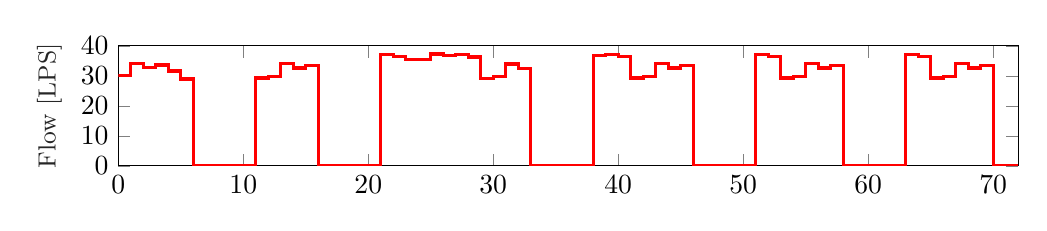
\begin{tikzpicture}

\begin{axis}[%
width=4.5in,
height=0.6in,
at={(0.948in,2.263in)},
scale only axis,
xmin=0,
xmax=72,
%xlabel style={font=\color{white!15!black}},
%xlabel={Time [h]},
ymin=0,
ymax=40,
ylabel style={font=\color{white!15!black}},
ylabel={\small Flow [LPS]},
axis background/.style={fill=white},
%title style={font=\bfseries},
%title={Inlet flows $\bar{d}_{\mathcal{K},1}$ and $\bar{d}_{\mathcal{K},2}$}
]
\addplot[const plot, color=red, line width=1.2pt, forget plot] table[row sep=crcr] {%
0	30.0046\\
1	34.1741\\
2	32.762\\
3	33.6315\\
4	31.5564\\
5	28.9859\\
6	0\\
7	0\\
8	0\\
9	0\\
10	0\\
11	29.2774\\
12	29.842\\
13	34.0029\\
14	32.5962\\
15	33.462\\
16	0\\
17	0\\
18	0\\
19	0\\
20	0\\
21	37.1075\\
22	36.3696\\
23	35.4455\\
24	35.4014\\
25	37.2252\\
26	36.6992\\
27	37.025\\
28	36.2878\\
29	29.2108\\
30	29.7754\\
31	33.9328\\
32	32.5282\\
33	0\\
34	0\\
35	0\\
36	0\\
37	0\\
38	36.7844\\
39	37.1088\\
40	36.371\\
41	29.2785\\
42	29.8431\\
43	34.0041\\
44	32.5973\\
45	33.4631\\
46	0\\
47	0\\
48	0\\
49	0\\
50	0\\
51	37.1071\\
52	36.3693\\
53	29.2771\\
54	29.8417\\
55	34.0026\\
56	32.5959\\
57	33.4617\\
58	0\\
59	0\\
60	0\\
61	0\\
62	0\\
63	37.1075\\
64	36.3696\\
65	29.2774\\
66	29.842\\
67	34.0029\\
68	32.5962\\
69	33.4619\\
70	0\\
71	0\\
72	0\\
};

\end{axis}
\end{tikzpicture}% 
 \vspace{-1.5mm}
 \caption{Inlet flows of the two pumping stations PU1 and PU2.}
 \label{fig:inlet_flows_example1}
 \end{figure}

\vspace{-3mm}

   %WT head
 \begin{figure}[H]
 \centering
 %
\includegraphics[width=0.35\textwidth]{report/pictures/missingfigure}
 % This file was created by matlab2tikz.
%
%The latest updates can be retrieved from
%  http://www.mathworks.com/matlabcentral/fileexchange/22022-matlab2tikz-matlab2tikz
%where you can also make suggestions and rate matlab2tikz.
%
\definecolor{mycolor1}{rgb}{0.00000,0.44700,0.74100}%
%
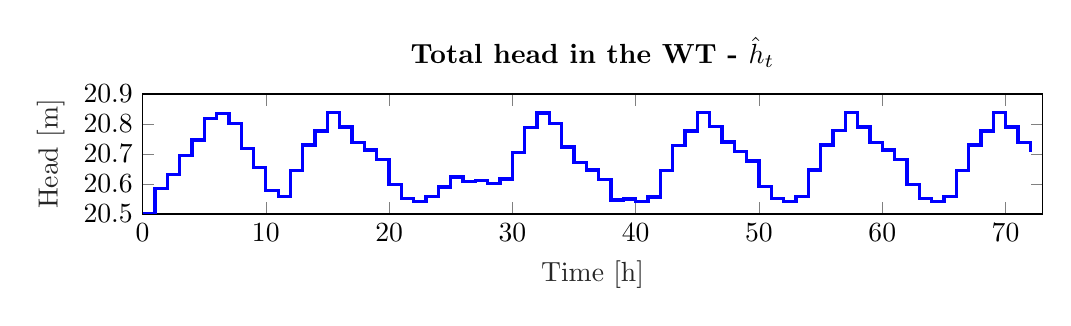
\begin{tikzpicture}

\begin{axis}[%
width=4.5in,
height=0.6in,
at={(0.761in,0.425in)},
scale only axis,
xmin=0,
xmax=73,
xlabel style={font=\color{white!15!black}},
xlabel={Time [h]},
ymin=20.5,
ymax=20.9,
ylabel style={font=\color{white!15!black}},
ylabel={Head  [m]},
axis background/.style={fill=white},
title style={font=\bfseries},
title={Total head in the WT - $\hat{h}_{t}$}
]
\addplot[const plot, color=blue, line width=1.2pt, forget plot] table[row sep=crcr] {%
0	20.5\\
1	20.5847\\
2	20.6325\\
3	20.6946\\
4	20.7469\\
5	20.8177\\
6	20.8338\\
7	20.8017\\
8	20.7183\\
9	20.6541\\
10	20.5771\\
11	20.5572\\
12	20.6458\\
13	20.7299\\
14	20.777\\
15	20.8386\\
16	20.79\\
17	20.7387\\
18	20.713\\
19	20.681\\
20	20.5975\\
21	20.5508\\
22	20.5419\\
23	20.5572\\
24	20.5901\\
25	20.6229\\
26	20.6078\\
27	20.6109\\
28	20.6018\\
29	20.617\\
30	20.7053\\
31	20.7891\\
32	20.836\\
33	20.8005\\
34	20.7235\\
35	20.6721\\
36	20.6465\\
37	20.6144\\
38	20.5466\\
39	20.5498\\
40	20.5409\\
41	20.5562\\
42	20.6448\\
43	20.7289\\
44	20.776\\
45	20.8376\\
46	20.7915\\
47	20.7402\\
48	20.7081\\
49	20.676\\
50	20.5926\\
51	20.5511\\
52	20.5421\\
53	20.5575\\
54	20.646\\
55	20.7301\\
56	20.7773\\
57	20.8388\\
58	20.7897\\
59	20.7383\\
60	20.7127\\
61	20.6806\\
62	20.5972\\
63	20.5509\\
64	20.5419\\
65	20.5572\\
66	20.6458\\
67	20.7299\\
68	20.777\\
69	20.8386\\
70	20.7901\\
71	20.7387\\
72	20.7066\\
};
\end{axis}
\end{tikzpicture}% 
 \vspace{-1.5mm}
 \caption{Head in the WT, TA1.}
 \label{fig:WT_head_example}
 \end{figure}

  %Sigma
 \begin{figure}[H]
 \centering
 %
\includegraphics[width=0.35\textwidth]{report/pictures/missingfigure}
 % This file was created by matlab2tikz.
%
%The latest updates can be retrieved from
%  http://www.mathworks.com/matlabcentral/fileexchange/22022-matlab2tikz-matlab2tikz
%where you can also make suggestions and rate matlab2tikz.
%
\definecolor{mycolor1}{rgb}{0.00000,0.44700,0.74100}%
%
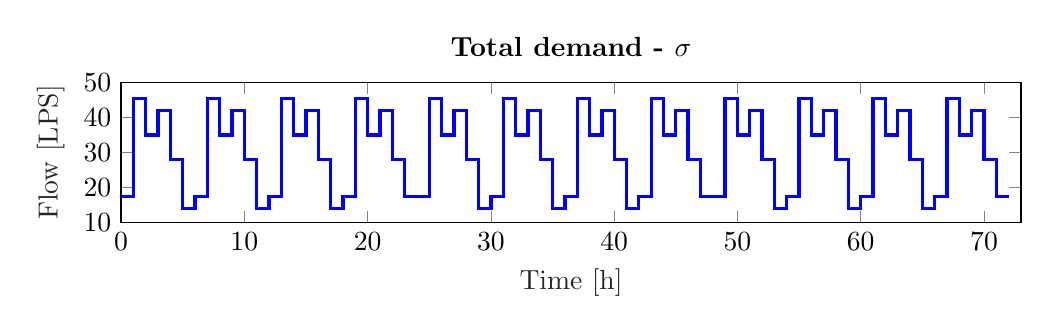
\begin{tikzpicture}

\begin{axis}[%
width=4.5in,
height=0.7in,
at={(0.784in,0.435in)},
scale only axis,
xmin=0,
xmax=73,
xlabel style={font=\color{white!15!black}},
xlabel={Time [h]},
ymin=10,
ymax=50,
ylabel style={font=\color{white!15!black}},
ylabel={Flow  [LPS]},
axis background/.style={fill=white},
title style={font=\bfseries},
title={Total demand - $\sigma$}
]
\addplot[const plot, color=blue, line width=1.2pt, forget plot] table[row sep=crcr] {%
0	17.5\\
1	45.5\\
2	35\\
3	42\\
4	28\\
5	14\\
6	17.5\\
7	45.5\\
8	35\\
9	42\\
10	28\\
11	14\\
12	17.5\\
13	45.5\\
14	35\\
15	42\\
16	28\\
17	14\\
18	17.5\\
19	45.5\\
20	35\\
21	42\\
22	28\\
23	17.5\\
24	17.5\\
25	45.5\\
26	35\\
27	42\\
28	28\\
29	14\\
30	17.5\\
31	45.5\\
32	35\\
33	42\\
34	28\\
35	14\\
36	17.5\\
37	45.5\\
38	35\\
39	42\\
40	28\\
41	14\\
42	17.5\\
43	45.5\\
44	35\\
45	42\\
46	28\\
47	17.5\\
48	17.5\\
49	45.5\\
50	35\\
51	42\\
52	28\\
53	14\\
54	17.5\\
55	45.5\\
56	35\\
57	42\\
58	28\\
59	14\\
60	17.5\\
61	45.5\\
62	35\\
63	42\\
64	28\\
65	14\\
66	17.5\\
67	45.5\\
68	35\\
69	42\\
70	28\\
71	17.5\\
72	17.5\\
};
\end{axis}
\end{tikzpicture}% 
 \vspace{-1.5mm}
 \caption{Total demand in the network.}
 \label{fig:sigma_example}
 \end{figure}

   %Inlet pressures
 \begin{figure}[H]
 \centering
 %
\includegraphics[width=0.35\textwidth]{report/pictures/missingfigure}
 % This file was created by matlab2tikz.
%
%The latest updates can be retrieved from
%  http://www.mathworks.com/matlabcentral/fileexchange/22022-matlab2tikz-matlab2tikz
%where you can also make suggestions and rate matlab2tikz.
%
\definecolor{mycolor1}{rgb}{0.00000,0.44700,0.74100}%
%
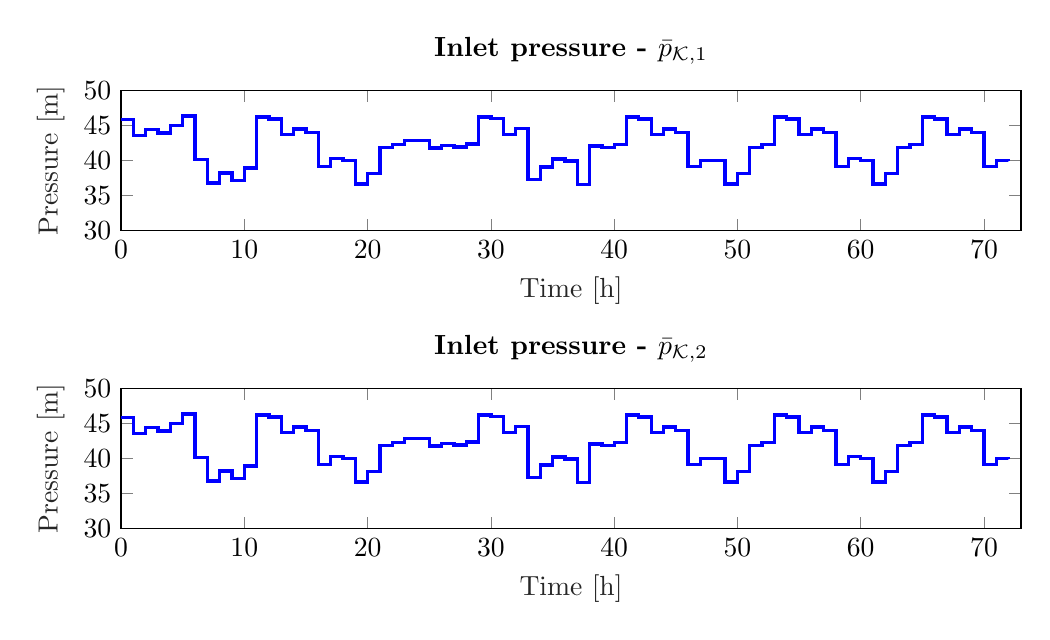
\begin{tikzpicture}

\begin{axis}[%
width=4.5in,
height=0.7in,
at={(0.892in,1.998in)},
scale only axis,
xmin=0,
xmax=73,
xlabel style={font=\color{white!15!black}},
xlabel={Time [h]},
ymin=30,
ymax=50,
ylabel style={font=\color{white!15!black}},
ylabel={Pressure  [m]},
axis background/.style={fill=white},
title style={font=\bfseries},
title={Inlet pressure - $\bar{p}_{\mathcal{K},1}$}
]
\addplot[const plot, color=blue, line width=1.2pt, forget plot] table[row sep=crcr] {%
0	45.8311\\
1	43.6012\\
2	44.3888\\
3	43.9077\\
4	45.035\\
5	46.3319\\
6	40.1154\\
7	36.7658\\
8	38.2118\\
9	37.1648\\
10	38.9031\\
11	46.1904\\
12	45.9122\\
13	43.6984\\
14	44.4791\\
15	44.0025\\
16	39.116\\
17	40.2569\\
18	39.9946\\
19	36.645\\
20	38.091\\
21	41.8587\\
22	42.3105\\
23	42.8635\\
24	42.8895\\
25	41.7857\\
26	42.1098\\
27	41.9096\\
28	42.36\\
29	46.2228\\
30	45.9453\\
31	43.7381\\
32	44.516\\
33	37.3111\\
34	39.0495\\
35	40.1904\\
36	39.928\\
37	36.5784\\
38	42.0576\\
39	41.8578\\
40	42.3096\\
41	46.1898\\
42	45.9116\\
43	43.6977\\
44	44.4785\\
45	44.0019\\
46	39.1175\\
47	40.0217\\
48	39.9897\\
49	36.64\\
50	38.0861\\
51	41.8589\\
52	42.3107\\
53	46.1905\\
54	45.9123\\
55	43.6986\\
56	44.4793\\
57	44.0027\\
58	39.1157\\
59	40.2566\\
60	39.9942\\
61	36.6446\\
62	38.0907\\
63	41.8587\\
64	42.3105\\
65	46.1904\\
66	45.9122\\
67	43.6984\\
68	44.4791\\
69	44.0025\\
70	39.1161\\
71	40.0203\\
72	39.9882\\
};
\end{axis}

\begin{axis}[%
width=4.5in,
height=0.7in,
at={(0.892in,0.508in)},
scale only axis,
xmin=0,
xmax=73,
xlabel style={font=\color{white!15!black}},
xlabel={Time [h]},
ymin=30,
ymax=50,
ylabel style={font=\color{white!15!black}},
ylabel={Pressure  [m]},
axis background/.style={fill=white},
title style={font=\bfseries},
title={Inlet pressure - $\bar{p}_{\mathcal{K},2}$}
]
\addplot[const plot, color=blue, line width=1.2pt, forget plot] table[row sep=crcr] {%
0	45.8311\\
1	43.6012\\
2	44.3888\\
3	43.9077\\
4	45.035\\
5	46.3319\\
6	40.1154\\
7	36.7658\\
8	38.2118\\
9	37.1648\\
10	38.9031\\
11	46.1904\\
12	45.9122\\
13	43.6984\\
14	44.4791\\
15	44.0025\\
16	39.116\\
17	40.2569\\
18	39.9946\\
19	36.645\\
20	38.091\\
21	41.8587\\
22	42.3105\\
23	42.8635\\
24	42.8895\\
25	41.7857\\
26	42.1098\\
27	41.9096\\
28	42.36\\
29	46.2228\\
30	45.9453\\
31	43.7381\\
32	44.516\\
33	37.3111\\
34	39.0495\\
35	40.1904\\
36	39.928\\
37	36.5784\\
38	42.0576\\
39	41.8578\\
40	42.3096\\
41	46.1898\\
42	45.9116\\
43	43.6977\\
44	44.4785\\
45	44.0019\\
46	39.1175\\
47	40.0217\\
48	39.9897\\
49	36.64\\
50	38.0861\\
51	41.8589\\
52	42.3107\\
53	46.1905\\
54	45.9123\\
55	43.6986\\
56	44.4793\\
57	44.0027\\
58	39.1157\\
59	40.2566\\
60	39.9942\\
61	36.6446\\
62	38.0907\\
63	41.8587\\
64	42.3105\\
65	46.1904\\
66	45.9122\\
67	43.6984\\
68	44.4791\\
69	44.0025\\
70	39.1161\\
71	40.0203\\
72	39.9882\\
};
\end{axis}
\end{tikzpicture}% 
 \vspace{-1.5mm}
 \caption{Inlet pressuresof the two pumping stations PU1 and PU2.}
 \label{fig:sigma_example}
 \end{figure}


